% Options for packages loaded elsewhere
\PassOptionsToPackage{unicode}{hyperref}
\PassOptionsToPackage{hyphens}{url}
\PassOptionsToPackage{dvipsnames,svgnames,x11names}{xcolor}
%
\documentclass[
  letterpaper,
]{article}

\usepackage{amsmath,amssymb}
\usepackage{iftex}
\ifPDFTeX
  \usepackage[T1]{fontenc}
  \usepackage[utf8]{inputenc}
  \usepackage{textcomp} % provide euro and other symbols
\else % if luatex or xetex
  \usepackage{unicode-math}
  \defaultfontfeatures{Scale=MatchLowercase}
  \defaultfontfeatures[\rmfamily]{Ligatures=TeX,Scale=1}
\fi
\usepackage{lmodern}
\ifPDFTeX\else  
    % xetex/luatex font selection
    \setmainfont[]{Liberation Sans}
    \setmonofont[Scale=0.8]{JetBrainsMono Nerd Font}
\fi
% Use upquote if available, for straight quotes in verbatim environments
\IfFileExists{upquote.sty}{\usepackage{upquote}}{}
\IfFileExists{microtype.sty}{% use microtype if available
  \usepackage[]{microtype}
  \UseMicrotypeSet[protrusion]{basicmath} % disable protrusion for tt fonts
}{}
\makeatletter
\@ifundefined{KOMAClassName}{% if non-KOMA class
  \IfFileExists{parskip.sty}{%
    \usepackage{parskip}
  }{% else
    \setlength{\parindent}{0pt}
    \setlength{\parskip}{6pt plus 2pt minus 1pt}}
}{% if KOMA class
  \KOMAoptions{parskip=half}}
\makeatother
\usepackage{xcolor}
\setlength{\emergencystretch}{3em} % prevent overfull lines
\setcounter{secnumdepth}{5}
% Make \paragraph and \subparagraph free-standing
\makeatletter
\ifx\paragraph\undefined\else
  \let\oldparagraph\paragraph
  \renewcommand{\paragraph}{
    \@ifstar
      \xxxParagraphStar
      \xxxParagraphNoStar
  }
  \newcommand{\xxxParagraphStar}[1]{\oldparagraph*{#1}\mbox{}}
  \newcommand{\xxxParagraphNoStar}[1]{\oldparagraph{#1}\mbox{}}
\fi
\ifx\subparagraph\undefined\else
  \let\oldsubparagraph\subparagraph
  \renewcommand{\subparagraph}{
    \@ifstar
      \xxxSubParagraphStar
      \xxxSubParagraphNoStar
  }
  \newcommand{\xxxSubParagraphStar}[1]{\oldsubparagraph*{#1}\mbox{}}
  \newcommand{\xxxSubParagraphNoStar}[1]{\oldsubparagraph{#1}\mbox{}}
\fi
\makeatother

\usepackage{color}
\usepackage{fancyvrb}
\newcommand{\VerbBar}{|}
\newcommand{\VERB}{\Verb[commandchars=\\\{\}]}
\DefineVerbatimEnvironment{Highlighting}{Verbatim}{commandchars=\\\{\}}
% Add ',fontsize=\small' for more characters per line
\usepackage{framed}
\definecolor{shadecolor}{RGB}{241,243,245}
\newenvironment{Shaded}{\begin{snugshade}}{\end{snugshade}}
\newcommand{\AlertTok}[1]{\textcolor[rgb]{0.68,0.00,0.00}{#1}}
\newcommand{\AnnotationTok}[1]{\textcolor[rgb]{0.37,0.37,0.37}{#1}}
\newcommand{\AttributeTok}[1]{\textcolor[rgb]{0.40,0.45,0.13}{#1}}
\newcommand{\BaseNTok}[1]{\textcolor[rgb]{0.68,0.00,0.00}{#1}}
\newcommand{\BuiltInTok}[1]{\textcolor[rgb]{0.00,0.23,0.31}{#1}}
\newcommand{\CharTok}[1]{\textcolor[rgb]{0.13,0.47,0.30}{#1}}
\newcommand{\CommentTok}[1]{\textcolor[rgb]{0.37,0.37,0.37}{#1}}
\newcommand{\CommentVarTok}[1]{\textcolor[rgb]{0.37,0.37,0.37}{\textit{#1}}}
\newcommand{\ConstantTok}[1]{\textcolor[rgb]{0.56,0.35,0.01}{#1}}
\newcommand{\ControlFlowTok}[1]{\textcolor[rgb]{0.00,0.23,0.31}{\textbf{#1}}}
\newcommand{\DataTypeTok}[1]{\textcolor[rgb]{0.68,0.00,0.00}{#1}}
\newcommand{\DecValTok}[1]{\textcolor[rgb]{0.68,0.00,0.00}{#1}}
\newcommand{\DocumentationTok}[1]{\textcolor[rgb]{0.37,0.37,0.37}{\textit{#1}}}
\newcommand{\ErrorTok}[1]{\textcolor[rgb]{0.68,0.00,0.00}{#1}}
\newcommand{\ExtensionTok}[1]{\textcolor[rgb]{0.00,0.23,0.31}{#1}}
\newcommand{\FloatTok}[1]{\textcolor[rgb]{0.68,0.00,0.00}{#1}}
\newcommand{\FunctionTok}[1]{\textcolor[rgb]{0.28,0.35,0.67}{#1}}
\newcommand{\ImportTok}[1]{\textcolor[rgb]{0.00,0.46,0.62}{#1}}
\newcommand{\InformationTok}[1]{\textcolor[rgb]{0.37,0.37,0.37}{#1}}
\newcommand{\KeywordTok}[1]{\textcolor[rgb]{0.00,0.23,0.31}{\textbf{#1}}}
\newcommand{\NormalTok}[1]{\textcolor[rgb]{0.00,0.23,0.31}{#1}}
\newcommand{\OperatorTok}[1]{\textcolor[rgb]{0.37,0.37,0.37}{#1}}
\newcommand{\OtherTok}[1]{\textcolor[rgb]{0.00,0.23,0.31}{#1}}
\newcommand{\PreprocessorTok}[1]{\textcolor[rgb]{0.68,0.00,0.00}{#1}}
\newcommand{\RegionMarkerTok}[1]{\textcolor[rgb]{0.00,0.23,0.31}{#1}}
\newcommand{\SpecialCharTok}[1]{\textcolor[rgb]{0.37,0.37,0.37}{#1}}
\newcommand{\SpecialStringTok}[1]{\textcolor[rgb]{0.13,0.47,0.30}{#1}}
\newcommand{\StringTok}[1]{\textcolor[rgb]{0.13,0.47,0.30}{#1}}
\newcommand{\VariableTok}[1]{\textcolor[rgb]{0.07,0.07,0.07}{#1}}
\newcommand{\VerbatimStringTok}[1]{\textcolor[rgb]{0.13,0.47,0.30}{#1}}
\newcommand{\WarningTok}[1]{\textcolor[rgb]{0.37,0.37,0.37}{\textit{#1}}}

\providecommand{\tightlist}{%
  \setlength{\itemsep}{0pt}\setlength{\parskip}{0pt}}\usepackage{longtable,booktabs,array}
\usepackage{calc} % for calculating minipage widths
% Correct order of tables after \paragraph or \subparagraph
\usepackage{etoolbox}
\makeatletter
\patchcmd\longtable{\par}{\if@noskipsec\mbox{}\fi\par}{}{}
\makeatother
% Allow footnotes in longtable head/foot
\IfFileExists{footnotehyper.sty}{\usepackage{footnotehyper}}{\usepackage{footnote}}
\makesavenoteenv{longtable}
\usepackage{graphicx}
\makeatletter
\def\maxwidth{\ifdim\Gin@nat@width>\linewidth\linewidth\else\Gin@nat@width\fi}
\def\maxheight{\ifdim\Gin@nat@height>\textheight\textheight\else\Gin@nat@height\fi}
\makeatother
% Scale images if necessary, so that they will not overflow the page
% margins by default, and it is still possible to overwrite the defaults
% using explicit options in \includegraphics[width, height, ...]{}
\setkeys{Gin}{width=\maxwidth,height=\maxheight,keepaspectratio}
% Set default figure placement to htbp
\makeatletter
\def\fps@figure{htbp}
\makeatother

\usepackage{booktabs}
\usepackage{longtable}
\usepackage{array}
\usepackage{multirow}
\usepackage{wrapfig}
\usepackage{float}
\usepackage{colortbl}
\usepackage{pdflscape}
\usepackage{tabu}
\usepackage{threeparttable}
\usepackage{threeparttablex}
\usepackage[normalem]{ulem}
\usepackage{makecell}
\usepackage{xcolor}
\newcommand{\fontmydefault}{\fontspec{Liberation Serif}}
\newcommand{\fontlibertsan}[1]{{\fontspec{Liberation Sans} #1}}
\newcommand{\fontlibertser}[1]{{\fontspec{Liberation Serif} #1}}
\newcommand{\fontlibertsnn}[1]{{\fontspec{Liberation Sans Narrow} #1}}
\newcommand{\fontnimbussan}[1]{{\fontspec{Nimbus Sans} #1}}
\newcommand{\fontnimbussnn}[1]{{\fontspec{Nimbus Sans Narrow} #1}}
\newcommand{\fontdejavusan}[1]{{\fontspec{DejaVu Sans} #1}}
\newcommand{\fontdejavuser}[1]{{\fontspec{DejaVu Serif} #1}}
\newcommand{\myfontchart}[1]{{\fontfamily{bch}\selectfont #1}}
\setlength{\defaultaddspace}{0pt} %This prevents tables in kable to display interpaces every 5 rows
\usepackage{wrapfig}
\usepackage{lipsum}
\usepackage{array}
\usepackage{float}
\usepackage{booktabs}
\usepackage{arydshln}
\usepackage{multirow}
\usepackage{xcolor}
\usepackage{tcolorbox}
\usepackage{geometry}
\geometry{ left=0.4in, right=0.4in, top=0.5in, bottom=0.5in}
\definecolor{pythoncol}{rgb}{0.188,0.412,0.596}
\definecolor{rcol}{rgb}{0.121,0.466,0.705}
\definecolor{bashcol}{rgb}{0.207,0.262,0.392}
\newtcolorbox{pythonheader}{ colback=pythoncol!70, colframe=pythoncol, fontupper=\footnotesize\bfseries\color{white}, boxrule=0.1mm, arc=4mm, left=1.5mm, right=1.5mm, top=0.5mm, bottom=0.5mm, halign=right, sharp corners=south}
\newtcolorbox{rheader}{ colback=rcol!70, colframe=rcol, fontupper=\footnotesize\bfseries\color{white}, boxrule=0.1mm, arc=4mm, left=1.5mm, right=1.5mm, top=0.5mm, bottom=0.5mm, halign=right, sharp corners=south}
\newtcolorbox{bashheader}{ colback=bashcol!70, colframe=bashcol, fontupper=\footnotesize\bfseries\color{white}, boxrule=0.1mm, arc=4mm, left=1.5mm, right=1.5mm, top=0.5mm, bottom=0.5mm, halign=right, sharp corners=south}
\newtcolorbox{testheader}[1]{ colback=red!5!white, colframe=red!75!black, fonttitle=\bfseries, title={#1}}
\newcolumntype{L}[1]{>{\raggedright\arraybackslash}p{#1}}
\newcolumntype{C}[1]{>{\centering\arraybackslash}p{#1}}
\newcolumntype{M}[1]{>{\centering\arraybackslash}m{#1}}
\newcolumntype{R}[1]{>{\raggedleft\arraybackslash}p{#1}}
\usepackage{pagecolor}
\definecolor{lightbeige}{RGB}{243,246,255}
\makeatletter
\@ifpackageloaded{caption}{}{\usepackage{caption}}
\AtBeginDocument{%
\ifdefined\contentsname
  \renewcommand*\contentsname{Table of contents}
\else
  \newcommand\contentsname{Table of contents}
\fi
\ifdefined\listfigurename
  \renewcommand*\listfigurename{List of Figures}
\else
  \newcommand\listfigurename{List of Figures}
\fi
\ifdefined\listtablename
  \renewcommand*\listtablename{List of Tables}
\else
  \newcommand\listtablename{List of Tables}
\fi
\ifdefined\figurename
  \renewcommand*\figurename{Figure}
\else
  \newcommand\figurename{Figure}
\fi
\ifdefined\tablename
  \renewcommand*\tablename{Table}
\else
  \newcommand\tablename{Table}
\fi
}
\@ifpackageloaded{float}{}{\usepackage{float}}
\floatstyle{ruled}
\@ifundefined{c@chapter}{\newfloat{codelisting}{h}{lop}}{\newfloat{codelisting}{h}{lop}[chapter]}
\floatname{codelisting}{Listing}
\newcommand*\listoflistings{\listof{codelisting}{List of Listings}}
\makeatother
\makeatletter
\makeatother
\makeatletter
\@ifpackageloaded{caption}{}{\usepackage{caption}}
\@ifpackageloaded{subcaption}{}{\usepackage{subcaption}}
\makeatother

\ifLuaTeX
  \usepackage{selnolig}  % disable illegal ligatures
\fi
\usepackage{bookmark}

\IfFileExists{xurl.sty}{\usepackage{xurl}}{} % add URL line breaks if available
\urlstyle{same} % disable monospaced font for URLs
\hypersetup{
  colorlinks=true,
  linkcolor={blue},
  filecolor={Maroon},
  citecolor={Blue},
  urlcolor={Blue},
  pdfcreator={LaTeX via pandoc}}


\author{}
\date{}

\begin{document}

\begin{titlepage}
\begin{flushleft}
  { UBMI-IFC, UNAM } \\
  { Coyoacan, CDMX }
\end{flushleft}
\vspace*{3cm}
\begin{center}
  { \Large Sequece Characterization Test } \\[1cm]
  { \large Using Genomic-Benchmarks Data }
\end{center}
\vfill
\begin{flushright}
\begin{tabular}{l@{\hspace*{\tabcolsep}}l}
  Author: & Fuentes David \\
  Tutors: & \\
  & - PhD. Poot Augusto \\
  & - MSc. Pedraza Carlos \\
\end{tabular}
\end{flushright}
\end{titlepage}

\renewcommand*\contentsname{Table of contents}
{
\hypersetup{linkcolor=}
\setcounter{tocdepth}{3}
\tableofcontents
}

\setlength\parindent{18pt}
\setlength\columnsep{18pt}
\newpage
\twocolumn

\section{Downloading data}\label{downloading-data}

\begin{pythonheader}
Python Code
\end{pythonheader}
\vspace{-1.75pt}

\begin{Shaded}
\begin{Highlighting}[]
\CommentTok{\# Note: Check \textquotesingle{}outputwrap\textquotesingle{} functions in source \textquotesingle{}qmd\textquotesingle{} }
\CommentTok{\#   notebook, for further insight on output display }

\CommentTok{\# To list available datasets}
\ImportTok{from}\NormalTok{ genomic\_benchmarks.data\_check }\ImportTok{import} \OperatorTok{\textbackslash{}}
\NormalTok{    list\_datasets}

\CommentTok{\# To inspect each dataset to select two}
\ImportTok{from}\NormalTok{ genomic\_benchmarks.data\_check }\ImportTok{import}\NormalTok{ info }\ImportTok{as} \OperatorTok{\textbackslash{}}
\NormalTok{    info\_gb}

\CommentTok{\# To download each dataset}
\ImportTok{from}\NormalTok{ genomic\_benchmarks.loc2seq }\ImportTok{import} \OperatorTok{\textbackslash{}}
\NormalTok{    download\_dataset}

\CommentTok{\# To position ourselves in the correct directory}
\ImportTok{import}\NormalTok{ os}
\end{Highlighting}
\end{Shaded}

\vspace{0.5cm}

\begin{Shaded}
\begin{Highlighting}[]
\NormalTok{list\_datasets()}
\end{Highlighting}
\end{Shaded}

\begin{verbatim}
['demo_human_or_worm',
'human_nontata_promoters',
'human_enhancers_ensembl',
'human_enhancers_cohn',
'dummy_mouse_enhancers_ensembl',
'demo_coding_vs_intergenomic_seqs',
'drosophila_enhancers_stark',
'human_ensembl_regulatory',
'human_ocr_ensembl']
\end{verbatim}

\vspace{0.5cm}

\begin{Shaded}
\begin{Highlighting}[]
\NormalTok{info\_gb(}\StringTok{"human\_nontata\_promoters"}\NormalTok{, version}\OperatorTok{=}\DecValTok{0}\NormalTok{)}
\end{Highlighting}
\end{Shaded}

\begin{verbatim}
Dataset `human_nontata_promoters` has 2 classes:
negative, positive.

 All lengths of genomic
intervals equals 251.

 Totally 36131 sequences
have been found, 27097 for training and 9034 for
testing.
          train  test
negative  12355  4119
positive  14742  4915
\end{verbatim}

\vspace{0.5cm}

\begin{Shaded}
\begin{Highlighting}[]
\NormalTok{info\_gb(}\StringTok{"human\_ensembl\_regulatory"}\NormalTok{, version}\OperatorTok{=}\DecValTok{0}\NormalTok{)}
\end{Highlighting}
\end{Shaded}

\begin{verbatim}
Dataset `human_ensembl_regulatory` has 3 classes:
enhancer, ocr, promoter.

 The length of genomic
intervals ranges from 71 to 802, with average
429.91753643694585 and median 401.0.

 Totally
289061 sequences have been found, 231348 for
training and 57713 for testing.
          train   test
enhancer  85512  21378
ocr       69902  17476
promoter  75934  18859
\end{verbatim}

\vspace{0.5cm}

\begin{Shaded}
\begin{Highlighting}[]
\NormalTok{info\_gb(}\StringTok{"human\_enhancers\_cohn"}\NormalTok{, version}\OperatorTok{=}\DecValTok{0}\NormalTok{)}
\end{Highlighting}
\end{Shaded}

\begin{verbatim}
Dataset `human_enhancers_cohn` has 2 classes:
negative, positive.

 All lengths of genomic
intervals equals 500.

 Totally 27791 sequences
have been found, 20843 for training and 6948 for
testing.
          train  test
negative  10422  3474
positive  10421  3474
\end{verbatim}

\vspace{0.5cm}

\begin{Shaded}
\begin{Highlighting}[]
\NormalTok{info\_gb(}\StringTok{"human\_enhancers\_ensembl"}\NormalTok{, version}\OperatorTok{=}\DecValTok{0}\NormalTok{)}
\end{Highlighting}
\end{Shaded}

\begin{verbatim}
Dataset `human_enhancers_ensembl` has 2 classes:
negative, positive.

 The length of genomic
intervals ranges from 2 to 573, with average
268.8641324705183 and median 269.0.

 Totally
154842 sequences have been found, 123872 for
training and 30970 for testing.
          train   test
negative  61936  15485
positive  61936  15485
\end{verbatim}

\vspace{0.5cm}

\begin{Shaded}
\begin{Highlighting}[]
\NormalTok{os.chdir(}\StringTok{"/path/to/Project/datasets/GenomicBenchmarks"}\NormalTok{)}

\NormalTok{download\_dataset(}\StringTok{"human\_nontata\_promoters"}\NormalTok{, version}\OperatorTok{=}\DecValTok{0}\NormalTok{) }
\NormalTok{download\_dataset(}\StringTok{"human\_enhancers\_cohn"}\NormalTok{, version}\OperatorTok{=}\DecValTok{0}\NormalTok{) }
\end{Highlighting}
\end{Shaded}

\newpage

\section{Formatting data}\label{formatting-data}

The downloaded data came in the form of two directories with many
\emph{.txt} files inside, and seeing that at least `\emph{getShape()}'
function from `\emph{DNAshapeR}' library required FASTA files to work
and it felt right to collect all sequences in a single file, I
transfered all sequences of each cis-regulatory element to their single
respective FASTA file and gave them a simple header.

\begin{bashheader}
Bash Code
\end{bashheader}
\vspace{-1.75pt}

\begin{Shaded}
\begin{Highlighting}[]
\BuiltInTok{cd}\NormalTok{ /path/to/Project/datasets/GenomicBenchmarks/}

\FunctionTok{awk} \StringTok{\textquotesingle{}BEGIN\{counter=0\}}
\StringTok{     \{print "\textgreater{}promoter\_"counter"|train|positive";}
\StringTok{     print $0; counter+=1\}\textquotesingle{}} \DataTypeTok{\textbackslash{}}
\NormalTok{     human\_nontata\_promoters/train/positive/}\PreprocessorTok{*}\NormalTok{.txt }\DataTypeTok{\textbackslash{}}
     \OperatorTok{\textgreater{}}\NormalTok{ promoters\_train\_positive.fasta}

\FunctionTok{awk} \StringTok{\textquotesingle{}BEGIN\{counter=0\}}
\StringTok{     \{print "\textgreater{}enhancer\_"counter"|train|positive"; }
\StringTok{     print $0; counter+=1\}\textquotesingle{}} \DataTypeTok{\textbackslash{}}
\NormalTok{     human\_enhancers\_cohn/train/positive/}\PreprocessorTok{*}\NormalTok{.txt }\DataTypeTok{\textbackslash{}}
     \OperatorTok{\textgreater{}}\NormalTok{ enhancers\_train\_positive.fasta}
\end{Highlighting}
\end{Shaded}

\section{Libraries used}\label{libraries-used}

Here is a list of the R libraries used for the following analysis, as
well as a reference to my own functions to be used in the
characterization step.

\begin{rheader}
R Code
\end{rheader}
\vspace{-1.75pt}

\begin{Shaded}
\begin{Highlighting}[]
\CommentTok{\# For genome{-}functions.R}
\FunctionTok{library}\NormalTok{(stringr)}
\FunctionTok{library}\NormalTok{(stringi)}
\FunctionTok{library}\NormalTok{(primes)}
\CommentTok{\# For parallel computing}
\FunctionTok{library}\NormalTok{(doParallel)}
\FunctionTok{library}\NormalTok{(foreach)}
\CommentTok{\# For biological functions: }
\CommentTok{\#   {-} Local/Global alignments }
\CommentTok{\#   {-} DNA Shape computing}
\FunctionTok{library}\NormalTok{(Biostrings)}
\FunctionTok{library}\NormalTok{(DNAshapeR)}
\CommentTok{\# For plotting}
\FunctionTok{library}\NormalTok{(paletteer)}
\FunctionTok{library}\NormalTok{(cowplot)}
\FunctionTok{library}\NormalTok{(ggplot2)}
\FunctionTok{library}\NormalTok{(dplyr)}
\FunctionTok{library}\NormalTok{(plyr)}
\FunctionTok{library}\NormalTok{(see)}
\CommentTok{\# For pretty tables}
\FunctionTok{library}\NormalTok{(knitr)}
\FunctionTok{library}\NormalTok{(kableExtra)}
\CommentTok{\# For my own functions}
\FunctionTok{source}\NormalTok{(}\StringTok{"/path/to/Project/scripts/genome{-}functions.R"}\NormalTok{)}
\end{Highlighting}
\end{Shaded}

\newpage

\section{Characterizing sequences}\label{characterizing-sequences}

Here, we characterize a subset from each of our datasets: 1638 sequences
per regulatory element; 3276 in total. However, there's a circumstance
about the sequences that has to be noted:

\begin{itemize}
\item
  Both datasets have considerably different elements lengthwise:

  \begin{enumerate}
  \def\labelenumi{\arabic{enumi}.}
  \item
    All promoters have a length of 251 nucleotides.
  \item
    All enhancers have a length of 500 nucleotides.
  \end{enumerate}
\item
  All features per sequence must be numerical and two-dimensional since
  we want it to be fed eventually to a simple classifier (like a Support
  Vector Machine).
\end{itemize}

\begin{Shaded}
\begin{Highlighting}[]
\NormalTok{proj\_path }\OtherTok{\textless{}{-}} \StringTok{"path/to/Project/datasets/GenomicBenchmarks"}
\NormalTok{prom\_fastaname }\OtherTok{\textless{}{-}} \StringTok{"promoters\_train\_positive.fasta"}
\NormalTok{enha\_fastaname }\OtherTok{\textless{}{-}} \StringTok{"enhancers\_train\_positive.fasta"}

\NormalTok{prom\_path }\OtherTok{\textless{}{-}} \FunctionTok{paste}\NormalTok{(proj\_path, prom\_fastaname, }\AttributeTok{sep =} \StringTok{"/"}\NormalTok{)}
\NormalTok{enha\_path }\OtherTok{\textless{}{-}} \FunctionTok{paste}\NormalTok{(proj\_path, enha\_fastaname, }\AttributeTok{sep =} \StringTok{"/"}\NormalTok{)}

\CommentTok{\# Scanning sequences}
\NormalTok{prom\_seqs }\OtherTok{\textless{}{-}} \FunctionTok{scan}\NormalTok{(prom\_path, }
                  \FunctionTok{character}\NormalTok{(), }\AttributeTok{quote=}\StringTok{""}\NormalTok{)[}\FunctionTok{seq}\NormalTok{(}\DecValTok{2}\NormalTok{,}\DecValTok{29484}\NormalTok{,}\DecValTok{2}\NormalTok{)]}
\NormalTok{enha\_seqs }\OtherTok{\textless{}{-}} \FunctionTok{scan}\NormalTok{(enha\_path, }
                  \FunctionTok{character}\NormalTok{(), }\AttributeTok{quote=}\StringTok{""}\NormalTok{)[}\FunctionTok{seq}\NormalTok{(}\DecValTok{2}\NormalTok{,}\DecValTok{20842}\NormalTok{,}\DecValTok{2}\NormalTok{)]}
\end{Highlighting}
\end{Shaded}

Given some previous tests done to `sequences\_characterizer()' I came to
the conclusion that parallel computing might provide a higher and more
complex set of data in a feasible time span.

\vspace{0.5cm}

\begin{Shaded}
\begin{Highlighting}[]
\CommentTok{\# Prepairing clusters for parallel computing}
\NormalTok{corescluster }\OtherTok{\textless{}{-}} \FunctionTok{makeCluster}\NormalTok{(}\DecValTok{6}\NormalTok{)}
\FunctionTok{registerDoParallel}\NormalTok{(corescluster)}

\CommentTok{\# Characterizing sequences and exporting to CSV}
\NormalTok{list\_seqs }\OtherTok{\textless{}{-}} \FunctionTok{list}\NormalTok{(}\AttributeTok{promoters =}\NormalTok{ prom\_seqs,}
                  \AttributeTok{enhancers =}\NormalTok{ enha\_seqs)}
\NormalTok{reg\_elems }\OtherTok{\textless{}{-}} \FunctionTok{c}\NormalTok{(}\StringTok{"promoters"}\NormalTok{, }\StringTok{"enhancers"}\NormalTok{)}
\NormalTok{libs }\OtherTok{\textless{}{-}} \FunctionTok{c}\NormalTok{(}\StringTok{"stringr"}\NormalTok{, }\StringTok{"stringi"}\NormalTok{, }\StringTok{"primes"}\NormalTok{)}

\ControlFlowTok{for}\NormalTok{ (reg\_elem }\ControlFlowTok{in}\NormalTok{ reg\_elems) \{}
  \FunctionTok{foreach}\NormalTok{(}\AttributeTok{i =} \DecValTok{1}\SpecialCharTok{:}\DecValTok{6}\NormalTok{) }\SpecialCharTok{\%dopar\%}\NormalTok{ \{}
    \FunctionTok{required\_libs}\NormalTok{(libs)}
\NormalTok{    i\_start }\OtherTok{\textless{}{-}}\NormalTok{ ((i }\SpecialCharTok{{-}} \DecValTok{1}\NormalTok{) }\SpecialCharTok{*} \DecValTok{273}\NormalTok{) }\SpecialCharTok{+} \DecValTok{1}
\NormalTok{    i\_final }\OtherTok{\textless{}{-}}\NormalTok{ i }\SpecialCharTok{*} \DecValTok{273}

    \ControlFlowTok{if}\NormalTok{ (i }\SpecialCharTok{\textgreater{}} \DecValTok{1}\NormalTok{) \{ }\CommentTok{\# Only the first CSV has headers}
      \FunctionTok{write.table}\NormalTok{(}
        \FunctionTok{sequences\_characterizer}\NormalTok{(}
\NormalTok{          list\_seqs[[reg\_elem]][i\_start}\SpecialCharTok{:}\NormalTok{i\_final],}
          \AttributeTok{optim =} \ConstantTok{TRUE}\NormalTok{, }\AttributeTok{k\_max =} \DecValTok{6}\NormalTok{),}
        \FunctionTok{paste}\NormalTok{(}
          \StringTok{"datasets/GB{-}Testing/test"}\NormalTok{, reg\_elem, }
          \StringTok{"{-}training\_"}\NormalTok{, i, }\StringTok{".csv"}\NormalTok{, }\AttributeTok{sep =} \StringTok{""}\NormalTok{), }
          \AttributeTok{row.names =} \ConstantTok{FALSE}\NormalTok{, }\AttributeTok{col.names =} \ConstantTok{FALSE}\NormalTok{,}
          \AttributeTok{sep =} \StringTok{","}\NormalTok{)}

\NormalTok{    \} }\ControlFlowTok{else}\NormalTok{ \{}
      \FunctionTok{write.csv}\NormalTok{(}
        \FunctionTok{sequences\_characterizer}\NormalTok{(}
\NormalTok{          list\_seqs[[reg\_elem]][i\_start}\SpecialCharTok{:}\NormalTok{i\_final],}
          \AttributeTok{optim =} \ConstantTok{TRUE}\NormalTok{, }\AttributeTok{k\_max =} \DecValTok{6}\NormalTok{),}
        \FunctionTok{paste}\NormalTok{(}
          \StringTok{"datasets/GB{-}Testing/"}\NormalTok{, reg\_elem,}
          \StringTok{"{-}training\_"}\NormalTok{, i, }\StringTok{".csv"}\NormalTok{, }\AttributeTok{sep =} \StringTok{""}\NormalTok{),}
          \AttributeTok{row.names =} \ConstantTok{FALSE}\NormalTok{)}
\NormalTok{\}\}\}}
\end{Highlighting}
\end{Shaded}

\section{Concatenating CSV's}\label{concatenating-csvs}

It was decided to produce many files instead of appending over the same
CSV table in order to apply a sort of quality control checkup after the
parallel computing was done. This, because when forcing the process RAM
overload was possible and the function could die mid-process. Since our
data was separated in six tables per cis-regulatory element, here we
only join each set together in a single CSV.

\begin{bashheader}
Bash Code
\end{bashheader}
\vspace{-1.75pt}

\begin{Shaded}
\begin{Highlighting}[]
\FunctionTok{cat}\NormalTok{ datasets/GB{-}Testing/testpromoters{-}training\_}\PreprocessorTok{*}\NormalTok{.csv }\DataTypeTok{\textbackslash{}}
    \OperatorTok{\textgreater{}}\NormalTok{ datasets/GB{-}Testing/test{-}1638{-}promoters{-}6mers.csv}
\FunctionTok{cat}\NormalTok{ datasets/GB{-}Testing/testenhancers{-}training\_}\PreprocessorTok{*}\NormalTok{.csv }\DataTypeTok{\textbackslash{}}
    \OperatorTok{\textgreater{}}\NormalTok{ datasets/GB{-}Testing/test{-}1638{-}enhancers{-}6mers.csv}
\end{Highlighting}
\end{Shaded}

\section{Data description}\label{data-description}

\begin{table}[h]
\caption{Overview of each column generated so far by '\textit{sequences-characterizer()}'}
\small
\centering
% Using the new column types L, C, and R for custom width and orientation
\begin{tabular}{|L{1.5cm}|C{2.5cm}|C{4cm}|} 
\hline
\centering \textbf{Column} & \textbf{Description} & \textbf{Section Processed} \\
\hline
A & \parbox[c][1.2cm]{2.5cm}{\centering Percentage of Alanines} & \multirow{6}{*}{\underline{per Sequence}} \\
\cdashline{1-2}
T & \parbox[c][1.2cm]{2.5cm}{\centering Percentage of Thymines} & \\
\cdashline{1-2}
C & \parbox[c][1.2cm]{2.5cm}{\centering Percentage of Cytosines} & \\
\cdashline{1-2}
G & \parbox[c][1.2cm]{2.5cm}{\centering Percentage of Guanines} & \\
\cdashline{1-2}
temp & \parbox[c][1.2cm]{2.5cm}{\centering Melting Temperature} & \\
\cdashline{1-2}
shan & \parbox[c][1.2cm]{2.5cm}{\centering Shannon Coefficient} & \\
\hline
kN.M\_prod & \parbox[c][1.25cm]{2.5cm}{\centering KSG Product} & \multirow{4}{*}{\parbox[t]{4cm}{
\setlength\parindent{35pt}\underline{per Kmer:}\\\\
each possible kmer of \\ size \textit{N}
is identified on a \\ scale of 1 to
$4^N$ denoted \\ by \textit{M}.\\\\
\texttt{
i.e. k3.1 (or the first\\
kmer of size 3) would be\\
AAA; k4.2 would be AAAC\\
}
}} \\
\cdashline{1-2}
kN.M\_barc & \parbox[c][1.2cm]{2.5cm}{\centering Barcode Profile} & \\
\cdashline{1-2}
kN.M\_pals & \parbox[c][1.2cm]{2.5cm}{\centering Palindrome Profile} & \\
\cdashline{1-2}
kN.M\_revc & \parbox[c][1.7cm]{2.5cm}{\centering Reverse Complement Profile} & \\
\hline
\end{tabular}
\end{table}

Prior to our primary analysis, it feels reasonable to explain the
columns per sequence produced by our tabulator
`\emph{sequences\_characterizer()}'. From here we'll first describe the
ones computed sequence-wise, the ones computed kmer-wise, then the ones
computed over each kmer distribution, and finally the ones corresponding
to DNA-Shape; this feature comes at last considering `\emph{getShape()}'
function makes its' own dataframe. The ones in \textbf{black} are
already integrated in the table, the ones in \color{red} \textbf{red}
\color{black} are yet to be adjoined:

\underline{Per sequence}

\begin{itemize}
\tightlist
\item
  From \emph{`genome-functions.R'}:

  \begin{itemize}
  \item
    \textbf{A, T, C, G} - \emph{Nucleotide Percentages} per sequence.
  \item
    \textbf{temp} - \textit{Melting \underline{Temp}erature}:
    Temperature at which DNA's double helix dissociates into single
    strands. \emph{It's dependent on GC percentage and sequence length.}
  \item
    \textbf{shan} - \textit{\underline{Shan}non Entropy Coefficient}:
    Statistical quantifier of information in a system. Measures the
    uncertainty a set of data has. In this case is a
    nucleotide-diversity metric. \emph{It's dependent on nucleotide
    percentages.}
  \end{itemize}
\item
  From \emph{`Biostrings'}:

  \begin{itemize}
  \item
    \color{red}\textbf{la\_sc} \color{black} -
    \textit{\underline{L}ocal \underline{A}lignment \underline{Sc}ore}
  \item
    \color{red}\textbf{la\_id} \color{black} -
    \textit{\underline{L}ocal \underline{A}lignment \underline{Id}entity}
  \item
    \color{red}\textbf{ga\_sc} \color{black} -
    \textit{\underline{G}lobal \underline{A}lignment \underline{Sc}ore}
  \item
    \color{red}\textbf{ga\_id} \color{black} -
    \textit{\underline{G}lobal \underline{A}lignment \underline{Id}entity}
  \end{itemize}
\end{itemize}

\underline{Per kmer}

Kmer characterization came with many challenges, principally to provide
each kmer with a distinct signature value dependent on their sequence
structure. This under the assumption that .

\begin{itemize}
\tightlist
\item
  From \emph{`genome-functions.R'}:

  \begin{itemize}
  \item
    \textbf{kN.M\_prod} - \textit{KSG \underline{Prod}uct}: Its obtained
    by multiplying \fontnimbussnn{\textbf{
      \underline{K}mer-Percentage * \underline{S}hannon Entropy * \underline{G}C-Percentage}}
    (\emph{in concept}). The justification for this comes from the
    desire to give each kmer a distictive signal based on their
    sequence. However many kmers can produce the same value depending on
    the function, for example, the kmers
    \fontnimbussnn{\textbf{'AAAT', 'ATAA', 'CCGC'}} and
    \fontnimbussnn{\textbf{'TGGG'}} all have the \emph{same Entropy
    Coefficient} (0.811), while
    \fontnimbussnn{\textbf{'GGAT', 'CAAG', 'AACC'}} and
    \fontnimbussnn{\textbf{'TGCT'}} all have the \emph{same GC
    Percentage} (0.5). Additionally, it is a little tricky to \emph{keep
    the product from becoming zero} when the sequence is either devoid
    of C/G nucleotides
    (e.g.~\textbf{\fontnimbussnn{gc\_percentage('ATTA')
      =0}}), or lacks nucleotide diversity
    (e.g.~\textbf{\fontnimbussnn{shannon\_entropy('GGGG')=0}}).
    \newline\small\fontlibertser{Refer to 'Theory \& Code Annex', Sections 2 \& 3, for more details.}\normalsize
  \item
    \textbf{kN.M\_barc} - \textit{\underline{Barc}ode Profile}: Its
    obtained by generating a vector with size equal to the kmer amount
    (which is equivalent to
    \fontnimbussnn{\textbf{'sequence length'} - \textbf{'kmer length'} + 1})
    and filling it with one prime number per cell in ascending order.
    Afterwars we use a logical (\fontnimbussnn{
      \textbf{1's \& 0's}}) vector of the same size to represent each
    kmer's positions in the sequence. \emph{In concept}, if we multiply
    both vectors we will get a set of prime numbers representing the
    positions of each kmer inside the sequence. If we multiply as well
    the elements inside this set, we will obtain an exlusive value for
    each kmer in each sequence, and only the sequences with the same
    kmers in the same place will be divisible by the corresponding
    prime.
  \item
    \textbf{kN.M\_pals} -
    \textit{\underline{Pal}indrome\underline{s}' Profile}:
  \item
    \textbf{kN.M\_revc} -
    \textit{\underline{Rev}erse \underline{C}omplement Profile}:
  \end{itemize}
\end{itemize}

\underline{Per kmer distribution}

\underline{Per non-defined kmer}

\begin{itemize}
\item
  From \emph{`DNAshapeR'}: \newline Generates a set features as vectors
  (EP, MGW, HelT, Roll \& ProT by default) per provided FASTA file.
  Splits each sequence in sliding kmers of size 5 (pentamers) not
  defined by me, which therefore makes vector size dependent on
  sequence-length. The features intended to be used are:

  \begin{itemize}
  \item
    \color{red}\textbf{sh\_ep} \color{black} - Shape EP
  \item
    \color{red}\textbf{sh\_mgw} \color{black} -
    \textit{\underline{M}inor \underline{G}roove \underline{W}idth}
  \item
    \color{red}\textbf{sh\_helt} \color{black} -
    \textit{\underline{Hel}ix \underline{T}wist}
  \item
    \color{red}\textbf{sh\_prot} \color{black} -
    \textit{\underline{Pro}peller \underline{T}wist}
  \item
    \color{red}\textbf{sh\_roll} \color{black} -
    \textit{\underline{Roll}}
  \end{itemize}
\end{itemize}

\section{Primary analysis}\label{primary-analysis}

Firstly we read our CSV tables into our conviniently named dataframes.

We could have concatenated both tables together, however I prefer to
keep them in different files.

\begin{rheader}
R Code
\end{rheader}
\vspace{-1.75pt}

\begin{Shaded}
\begin{Highlighting}[]
\FunctionTok{setwd}\NormalTok{(}\StringTok{"/path/to/Project/"}\NormalTok{)}
\NormalTok{testdir\_path }\OtherTok{\textless{}{-}} \StringTok{"datasets/GB{-}Testing/"}
\NormalTok{prom\_csvpath }\OtherTok{\textless{}{-}} \StringTok{"test{-}1638{-}promoters{-}6mers.csv"} 
\NormalTok{enha\_csvname }\OtherTok{\textless{}{-}} \StringTok{"test{-}1638{-}enhancers{-}6mers.csv"} 

\NormalTok{proms }\OtherTok{\textless{}{-}} \FunctionTok{read.csv}\NormalTok{(}\FunctionTok{paste0}\NormalTok{(testdir\_path, }
\NormalTok{                         prom\_csvname),}
                         \AttributeTok{check.names =}\NormalTok{ F)}
\NormalTok{enhas }\OtherTok{\textless{}{-}} \FunctionTok{read.csv}\NormalTok{(}\FunctionTok{paste0}\NormalTok{(testdir\_path, }
\NormalTok{                         enha\_csvname),}
                         \AttributeTok{check.names =}\NormalTok{ F)}
\NormalTok{CREs }\OtherTok{\textless{}{-}} \FunctionTok{c}\NormalTok{(}\StringTok{"Promoter"}\NormalTok{,}\StringTok{"Enhancer"}\NormalTok{)}
\end{Highlighting}
\end{Shaded}

\vspace{0.2cm}

First we get an overviwew of the dimensions of our data: NOTE: Replace
this with some kind of table \vspace{0.2cm}

\begin{Shaded}
\begin{Highlighting}[]
\FunctionTok{deparse}\NormalTok{(}\FunctionTok{substitute}\NormalTok{(proms))}
\FunctionTok{deparse}\NormalTok{(}\FunctionTok{substitute}\NormalTok{(enhas))}
\FunctionTok{dim}\NormalTok{(proms)}
\FunctionTok{dim}\NormalTok{(enhas)}
\end{Highlighting}
\end{Shaded}

\begin{figure}

\begin{minipage}{0.50\linewidth}

\begin{verbatim}
[1] "proms"
\end{verbatim}

\end{minipage}%
%
\begin{minipage}{0.50\linewidth}

\begin{verbatim}
[1] "enhas"
\end{verbatim}

\end{minipage}%
\newline
\begin{minipage}{0.50\linewidth}

\begin{verbatim}
[1]  1638 21830
\end{verbatim}

\end{minipage}%
%
\begin{minipage}{0.50\linewidth}

\begin{verbatim}
[1]  1638 21830
\end{verbatim}

\end{minipage}%

\end{figure}%

\vspace{0.2cm}

It's noticeable the fact that we have way more columns than rows in this
test table. Let's get a general glimpse of the first three promoters'
rows by displaying the first 3 lines and first 18 columns pertaining to
all \emph{sequence-wise} variables computed so far plus the first 12
\emph{kmer-wise} variables, which align with the data related to the
first 3 kmers (\fontnimbussnn{\textbf{'AA', 'AC'} \& \textbf{'AG'}}):

\vspace{0.2cm}

\begin{Shaded}
\begin{Highlighting}[]
\FunctionTok{teatable}\NormalTok{(proms[}\DecValTok{1}\SpecialCharTok{:}\DecValTok{3}\NormalTok{,}\DecValTok{1}\SpecialCharTok{:}\DecValTok{18}\NormalTok{])}
\end{Highlighting}
\end{Shaded}

\begin{table}[!h]
\footnotesize
\centering
\resizebox{\ifdim\width>\linewidth\linewidth\else\width\fi}{!}{
\begin{tabular}[t]{>{\centering\arraybackslash}p{5.75em}>{\centering\arraybackslash}p{5.75em}>{\centering\arraybackslash}p{5.75em}>{\centering\arraybackslash}p{5.75em}>{\centering\arraybackslash}p{5.75em}>{\centering\arraybackslash}p{5.75em}}
\specialrule{1pt}{0pt}{1pt}
\cellcolor[HTML]{ccccb3}{A} & \cellcolor[HTML]{ccccb3}{T} & \cellcolor[HTML]{ccccb3}{C} & \cellcolor[HTML]{ccccb3}{G} & \cellcolor[HTML]{ccccb3}{temp} & \cellcolor[HTML]{ccccb3}{shan}\\
\specialrule{0.6pt}{0.8pt}{0.6pt}
\cellcolor[HTML]{e0e0cc}{0.1673307} & \cellcolor[HTML]{e0e0cc}{0.2231076} & \cellcolor[HTML]{e0e0cc}{0.3306773} & \cellcolor[HTML]{e0e0cc}{0.2788845} & \cellcolor[HTML]{e0e0cc}{87.21315} & \cellcolor[HTML]{e0e0cc}{1.956136}\\
\cellcolor[HTML]{f4f4e2}{0.2629482} & \cellcolor[HTML]{f4f4e2}{0.2788845} & \cellcolor[HTML]{f4f4e2}{0.2549801} & \cellcolor[HTML]{f4f4e2}{0.2031873} & \cellcolor[HTML]{f4f4e2}{81.00598} & \cellcolor[HTML]{f4f4e2}{1.990374}\\
\cellcolor[HTML]{e0e0cc}{0.3625498} & \cellcolor[HTML]{e0e0cc}{0.2031873} & \cellcolor[HTML]{e0e0cc}{0.2470120} & \cellcolor[HTML]{e0e0cc}{0.1872510} & \cellcolor[HTML]{e0e0cc}{80.02590} & \cellcolor[HTML]{e0e0cc}{1.948719}\\
\specialrule{1pt}{0.6pt}{0pt}
\end{tabular}}
\end{table}

\begin{table}[!h]
\footnotesize
\centering
\resizebox{\ifdim\width>\linewidth\linewidth\else\width\fi}{!}{
\begin{tabular}[t]{>{\centering\arraybackslash}p{5.75em}>{\centering\arraybackslash}p{5.75em}>{\centering\arraybackslash}p{5.75em}>{\centering\arraybackslash}p{5.75em}>{\centering\arraybackslash}p{5.75em}>{\centering\arraybackslash}p{5.75em}}
\specialrule{1pt}{0pt}{1pt}
\cellcolor[HTML]{ccccb3}{k2.1\_prod} & \cellcolor[HTML]{ccccb3}{k2.1\_barc} & \cellcolor[HTML]{ccccb3}{k2.1\_pals} & \cellcolor[HTML]{ccccb3}{k2.1\_revc} & \cellcolor[HTML]{ccccb3}{k2.2\_prod} & \cellcolor[HTML]{ccccb3}{k2.2\_barc}\\
\specialrule{0.6pt}{0.8pt}{0.6pt}
\cellcolor[HTML]{e0e0cc}{9} & \cellcolor[HTML]{e0e0cc}{1.959765} & \cellcolor[HTML]{e0e0cc}{2.177403e+09} & \cellcolor[HTML]{e0e0cc}{1.374020e+12} & \cellcolor[HTML]{e0e0cc}{17.11198} & \cellcolor[HTML]{e0e0cc}{1.531862}\\
\cellcolor[HTML]{f4f4e2}{17} & \cellcolor[HTML]{f4f4e2}{2.633165} & \cellcolor[HTML]{f4f4e2}{1.138401e+17} & \cellcolor[HTML]{f4f4e2}{2.971115e+17} & \cellcolor[HTML]{f4f4e2}{26.44579} & \cellcolor[HTML]{f4f4e2}{2.624612}\\
\cellcolor[HTML]{e0e0cc}{38} & \cellcolor[HTML]{e0e0cc}{5.347025} & \cellcolor[HTML]{e0e0cc}{3.981015e+36} & \cellcolor[HTML]{e0e0cc}{8.100763e+29} & \cellcolor[HTML]{e0e0cc}{24.89016} & \cellcolor[HTML]{e0e0cc}{1.855662}\\
\specialrule{1pt}{0.6pt}{0pt}
\end{tabular}}
\end{table}

\begin{table}[!h]
\footnotesize
\centering
\resizebox{\ifdim\width>\linewidth\linewidth\else\width\fi}{!}{
\begin{tabular}[t]{>{\centering\arraybackslash}p{5.75em}>{\centering\arraybackslash}p{5.75em}>{\centering\arraybackslash}p{5.75em}>{\centering\arraybackslash}p{5.75em}>{\centering\arraybackslash}p{5.75em}>{\centering\arraybackslash}p{5.75em}}
\specialrule{1pt}{0pt}{1pt}
\cellcolor[HTML]{ccccb3}{k2.2\_pals} & \cellcolor[HTML]{ccccb3}{k2.2\_revc} & \cellcolor[HTML]{ccccb3}{k2.3\_prod} & \cellcolor[HTML]{ccccb3}{k2.3\_barc} & \cellcolor[HTML]{ccccb3}{k2.3\_pals} & \cellcolor[HTML]{ccccb3}{k2.3\_revc}\\
\specialrule{0.6pt}{0.8pt}{0.6pt}
\cellcolor[HTML]{e0e0cc}{3.845422e+15} & \cellcolor[HTML]{e0e0cc}{3.525451e+11} & \cellcolor[HTML]{e0e0cc}{26.44579} & \cellcolor[HTML]{e0e0cc}{2.445328} & \cellcolor[HTML]{e0e0cc}{4.788062e+13} & \cellcolor[HTML]{e0e0cc}{1.305836e+26}\\
\cellcolor[HTML]{f4f4e2}{2.607331e+20} & \cellcolor[HTML]{f4f4e2}{6.308689e+14} & \cellcolor[HTML]{f4f4e2}{24.89016} & \cellcolor[HTML]{f4f4e2}{2.513656} & \cellcolor[HTML]{f4f4e2}{1.320117e+14} & \cellcolor[HTML]{f4f4e2}{6.435389e+19}\\
\cellcolor[HTML]{e0e0cc}{1.156904e+25} & \cellcolor[HTML]{e0e0cc}{3.573059e+12} & \cellcolor[HTML]{e0e0cc}{34.22397} & \cellcolor[HTML]{e0e0cc}{3.431445} & \cellcolor[HTML]{e0e0cc}{6.011592e+17} & \cellcolor[HTML]{e0e0cc}{7.178542e+17}\\
\specialrule{1pt}{0.6pt}{0pt}
\end{tabular}}
\end{table}

\vspace{0.2cm}

We'll get a similar panorama when looking at the first three enhancers'
rows (although it seems like \emph{`barcode'} values appear to be
significantly larger):

\vspace{0.2cm}

\begin{Shaded}
\begin{Highlighting}[]
\FunctionTok{teatable}\NormalTok{(enhas[}\DecValTok{1}\SpecialCharTok{:}\DecValTok{3}\NormalTok{,}\DecValTok{1}\SpecialCharTok{:}\DecValTok{18}\NormalTok{])}
\end{Highlighting}
\end{Shaded}

\begin{table}[!h]
\footnotesize
\centering
\resizebox{\ifdim\width>\linewidth\linewidth\else\width\fi}{!}{
\begin{tabular}[t]{>{\centering\arraybackslash}p{6em}>{\centering\arraybackslash}p{6em}>{\centering\arraybackslash}p{6em}>{\centering\arraybackslash}p{6em}>{\centering\arraybackslash}p{6em}>{\centering\arraybackslash}p{6em}}
\specialrule{1pt}{0pt}{1pt}
\cellcolor[HTML]{ccccb3}{A} & \cellcolor[HTML]{ccccb3}{T} & \cellcolor[HTML]{ccccb3}{C} & \cellcolor[HTML]{ccccb3}{G} & \cellcolor[HTML]{ccccb3}{temp} & \cellcolor[HTML]{ccccb3}{shan}\\
\specialrule{0.6pt}{0.8pt}{0.6pt}
\cellcolor[HTML]{e0e0cc}{0.240} & \cellcolor[HTML]{e0e0cc}{0.236} & \cellcolor[HTML]{e0e0cc}{0.234} & \cellcolor[HTML]{e0e0cc}{0.290} & \cellcolor[HTML]{e0e0cc}{85.0392} & \cellcolor[HTML]{e0e0cc}{1.993988}\\
\cellcolor[HTML]{f4f4e2}{0.204} & \cellcolor[HTML]{f4f4e2}{0.286} & \cellcolor[HTML]{f4f4e2}{0.210} & \cellcolor[HTML]{f4f4e2}{0.300} & \cellcolor[HTML]{f4f4e2}{84.4652} & \cellcolor[HTML]{f4f4e2}{1.978249}\\
\cellcolor[HTML]{e0e0cc}{0.250} & \cellcolor[HTML]{e0e0cc}{0.280} & \cellcolor[HTML]{e0e0cc}{0.258} & \cellcolor[HTML]{e0e0cc}{0.212} & \cellcolor[HTML]{e0e0cc}{82.8252} & \cellcolor[HTML]{e0e0cc}{1.992923}\\
\specialrule{1pt}{0.6pt}{0pt}
\end{tabular}}
\end{table}

\begin{table}[!h]
\footnotesize
\centering
\resizebox{\ifdim\width>\linewidth\linewidth\else\width\fi}{!}{
\begin{tabular}[t]{>{\centering\arraybackslash}p{6em}>{\centering\arraybackslash}p{6em}>{\centering\arraybackslash}p{6em}>{\centering\arraybackslash}p{6em}>{\centering\arraybackslash}p{6em}>{\centering\arraybackslash}p{6em}}
\specialrule{1pt}{0pt}{1pt}
\cellcolor[HTML]{ccccb3}{k2.1\_prod} & \cellcolor[HTML]{ccccb3}{k2.1\_barc} & \cellcolor[HTML]{ccccb3}{k2.1\_pals} & \cellcolor[HTML]{ccccb3}{k2.1\_revc} & \cellcolor[HTML]{ccccb3}{k2.2\_prod} & \cellcolor[HTML]{ccccb3}{k2.2\_barc}\\
\specialrule{0.6pt}{0.8pt}{0.6pt}
\cellcolor[HTML]{e0e0cc}{36} & \cellcolor[HTML]{e0e0cc}{10.432345} & \cellcolor[HTML]{e0e0cc}{1.885437e+37} & \cellcolor[HTML]{e0e0cc}{8.632413e+30} & \cellcolor[HTML]{e0e0cc}{24.89016} & \cellcolor[HTML]{e0e0cc}{6.027803}\\
\cellcolor[HTML]{f4f4e2}{20} & \cellcolor[HTML]{f4f4e2}{6.153015} & \cellcolor[HTML]{f4f4e2}{5.673403e+20} & \cellcolor[HTML]{f4f4e2}{1.061673e+53} & \cellcolor[HTML]{f4f4e2}{23.33452} & \cellcolor[HTML]{f4f4e2}{4.984254}\\
\cellcolor[HTML]{e0e0cc}{31} & \cellcolor[HTML]{e0e0cc}{9.936447} & \cellcolor[HTML]{e0e0cc}{1.640775e+32} & \cellcolor[HTML]{e0e0cc}{5.563175e+39} & \cellcolor[HTML]{e0e0cc}{46.66905} & \cellcolor[HTML]{e0e0cc}{9.301359}\\
\specialrule{1pt}{0.6pt}{0pt}
\end{tabular}}
\end{table}

\begin{table}[!h]
\footnotesize
\centering
\resizebox{\ifdim\width>\linewidth\linewidth\else\width\fi}{!}{
\begin{tabular}[t]{>{\centering\arraybackslash}p{6em}>{\centering\arraybackslash}p{6em}>{\centering\arraybackslash}p{6em}>{\centering\arraybackslash}p{6em}>{\centering\arraybackslash}p{6em}>{\centering\arraybackslash}p{6em}}
\specialrule{1pt}{0pt}{1pt}
\cellcolor[HTML]{ccccb3}{k2.2\_pals} & \cellcolor[HTML]{ccccb3}{k2.2\_revc} & \cellcolor[HTML]{ccccb3}{k2.3\_prod} & \cellcolor[HTML]{ccccb3}{k2.3\_barc} & \cellcolor[HTML]{ccccb3}{k2.3\_pals} & \cellcolor[HTML]{ccccb3}{k2.3\_revc}\\
\specialrule{0.6pt}{0.8pt}{0.6pt}
\cellcolor[HTML]{e0e0cc}{1.579134e+29} & \cellcolor[HTML]{e0e0cc}{1.707234e+31} & \cellcolor[HTML]{e0e0cc}{76.22611} & \cellcolor[HTML]{e0e0cc}{13.43518} & \cellcolor[HTML]{e0e0cc}{3.557032e+41} & \cellcolor[HTML]{e0e0cc}{5.830130e+44}\\
\cellcolor[HTML]{f4f4e2}{4.485619e+32} & \cellcolor[HTML]{f4f4e2}{1.810188e+35} & \cellcolor[HTML]{f4f4e2}{73.11484} & \cellcolor[HTML]{f4f4e2}{13.29662} & \cellcolor[HTML]{f4f4e2}{3.273426e+39} & \cellcolor[HTML]{f4f4e2}{3.755909e+39}\\
\cellcolor[HTML]{e0e0cc}{9.951038e+37} & \cellcolor[HTML]{e0e0cc}{3.612544e+25} & \cellcolor[HTML]{e0e0cc}{60.66976} & \cellcolor[HTML]{e0e0cc}{12.53356} & \cellcolor[HTML]{e0e0cc}{4.255600e+33} & \cellcolor[HTML]{e0e0cc}{3.010280e+57}\\
\specialrule{1pt}{0.6pt}{0pt}
\end{tabular}}
\end{table}

\begin{Shaded}
\begin{Highlighting}[]
\NormalTok{mean\_prom }\OtherTok{\textless{}{-}} \FunctionTok{colMeans}\NormalTok{(proms)}
\NormalTok{mean\_enha }\OtherTok{\textless{}{-}} \FunctionTok{colMeans}\NormalTok{(enhas)}
\NormalTok{sd\_prom }\OtherTok{\textless{}{-}} \FunctionTok{apply}\NormalTok{(proms, }\DecValTok{2}\NormalTok{, sd)}
\NormalTok{sd\_enha }\OtherTok{\textless{}{-}} \FunctionTok{apply}\NormalTok{(enhas, }\DecValTok{2}\NormalTok{, sd)}

\NormalTok{names\_CREs }\OtherTok{\textless{}{-}} \FunctionTok{rep}\NormalTok{(CREs, }\AttributeTok{each =} \FunctionTok{length}\NormalTok{(proms))}
\NormalTok{cre\_summary }\OtherTok{\textless{}{-}} \FunctionTok{data.frame}\NormalTok{(}\AttributeTok{Type =} \FunctionTok{factor}\NormalTok{(names\_CREs),}
                          \AttributeTok{Field =} \FunctionTok{rep}\NormalTok{(}\FunctionTok{names}\NormalTok{(proms),}\DecValTok{2}\NormalTok{),}
                          \AttributeTok{Means =} \FunctionTok{c}\NormalTok{(mean\_prom,mean\_enha),}
                          \AttributeTok{StDevs =} \FunctionTok{c}\NormalTok{(sd\_prom,sd\_enha))}
\end{Highlighting}
\end{Shaded}

\begin{Shaded}
\begin{Highlighting}[]
\NormalTok{ldf }\OtherTok{\textless{}{-}} \FunctionTok{length}\NormalTok{(proms)}
\FunctionTok{coffeetable}\NormalTok{(cre\_summary[}\FunctionTok{c}\NormalTok{(}\DecValTok{1}\SpecialCharTok{:}\DecValTok{10}\NormalTok{,(ldf}\SpecialCharTok{+}\DecValTok{1}\NormalTok{)}\SpecialCharTok{:}\NormalTok{(ldf}\SpecialCharTok{+}\DecValTok{10}\NormalTok{)),])}
\end{Highlighting}
\end{Shaded}

\begin{table}[!h]
\centering
\footnotesize
\renewcommand{\arraystretch}{1.3}
\resizebox{\ifdim\width>\linewidth\linewidth\else\width\fi}{!}{
\begin{tabular}[t]{lllrr}
\specialrule{1pt}{0pt}{0.5pt}
\rowcolor{brown!42}
  & Type & Field & Means & StDevs\\
\specialrule{0.6pt}{1pt}{0pt}
\rowcolor{brown!25}
1 & \cellcolor{brown!10} & A & 1.911256e-01 & 7.145510e-02\\[-0.12pt]
\rowcolor{brown!10}
2 & \cellcolor{brown!10} & T & 1.995826e-01 & 7.599340e-02\\[-0.12pt]
\rowcolor{brown!25}
3 & \cellcolor{brown!10} & C & 2.962655e-01 & 8.067840e-02\\[-0.12pt]
\rowcolor{brown!10}
4 & \cellcolor{brown!10} & G & 3.130263e-01 & 8.524230e-02\\[-0.12pt]
\rowcolor{brown!25}
5 & \cellcolor{brown!10} & temp & 8.720208e+01 & 5.379461e+00\\[-0.12pt]
\rowcolor{brown!10}
6 & \cellcolor{brown!10} & shan & 1.891724e+00 & 9.437000e-02\\[-0.12pt]
\rowcolor{brown!25}
7 & \cellcolor{brown!10} & k2.1\_prod & 1.196276e+01 & 8.995306e+00\\[-0.12pt]
\rowcolor{brown!10}
8 & \cellcolor{brown!10} & k2.1\_barc & 1.500971e+00 & 1.229003e+00\\[-0.12pt]
\rowcolor{brown!25}
9 & \cellcolor{brown!10} & k2.1\_pals & 2.634405e+51 & 1.065029e+53\\[-0.12pt]
\rowcolor{brown!10}
10 & \multirow{-10}{*}{\raggedright\arraybackslash\cellcolor{brown!10} Promoter} & k2.1\_revc & 9.789346e+62 & 3.960331e+64\\[-0.12pt]
\rowcolor{brown!25}
21831 & \cellcolor{brown!25} & A & 2.653712e-01 & 5.853000e-02\\[-0.12pt]
\rowcolor{brown!10}
21832 & \cellcolor{brown!25} & T & 2.678205e-01 & 5.815610e-02\\[-0.12pt]
\rowcolor{brown!25}
21833 & \cellcolor{brown!25} & C & 2.351111e-01 & 5.648440e-02\\[-0.12pt]
\rowcolor{brown!10}
21834 & \cellcolor{brown!25} & G & 2.316972e-01 & 5.435370e-02\\[-0.12pt]
\rowcolor{brown!25}
21835 & \cellcolor{brown!25} & temp & 8.269434e+01 & 3.785299e+00\\[-0.12pt]
\rowcolor{brown!10}
21836 & \cellcolor{brown!25} & shan & 1.959202e+00 & 3.892580e-02\\[-0.12pt]
\rowcolor{brown!25}
21837 & \cellcolor{brown!25} & k2.1\_prod & 4.093346e+01 & 1.835697e+01\\[-0.12pt]
\rowcolor{brown!10}
21838 & \cellcolor{brown!25} & k2.1\_barc & 1.208127e+01 & 5.751107e+00\\[-0.12pt]
\rowcolor{brown!25}
21839 & \cellcolor{brown!25} & k2.1\_pals & 2.567318e+112 & 1.038419e+114\\[-0.12pt]
\rowcolor{brown!10}
21840 & \multirow{-10}{*}{\raggedright\arraybackslash\cellcolor{brown!25} Enhancer} & k2.1\_revc & 3.321646e+121 & 1.344343e+123\\[-0.12pt]
\bottomrule
\end{tabular}}
\renewcommand{\arraystretch}{1}

\end{table}

\begin{Shaded}
\begin{Highlighting}[]
\CommentTok{\# Get only \textquotesingle{}prod\textquotesingle{} columns of each kmer}

\NormalTok{k\_Ns }\OtherTok{\textless{}{-}} \FunctionTok{c}\NormalTok{(}\FunctionTok{n\_ki}\NormalTok{(}\DecValTok{2}\NormalTok{), }\FunctionTok{n\_ki}\NormalTok{(}\DecValTok{3}\NormalTok{), }\FunctionTok{n\_ki}\NormalTok{(}\DecValTok{4}\NormalTok{), }\FunctionTok{n\_ki}\NormalTok{(}\DecValTok{5}\NormalTok{), }\FunctionTok{n\_ki}\NormalTok{(}\DecValTok{6}\NormalTok{)) }
\NormalTok{k\_inds }\OtherTok{\textless{}{-}} \FunctionTok{c}\NormalTok{(}\DecValTok{0}\NormalTok{)}
\ControlFlowTok{for}\NormalTok{ (k\_n }\ControlFlowTok{in}\NormalTok{ k\_Ns) \{}
\NormalTok{  k\_inds }\OtherTok{\textless{}{-}} \FunctionTok{c}\NormalTok{(k\_inds, }\FunctionTok{tail}\NormalTok{(k\_inds,}\DecValTok{1}\NormalTok{) }\SpecialCharTok{+} \DecValTok{1}\NormalTok{)}
\NormalTok{  k\_inds }\OtherTok{\textless{}{-}} \FunctionTok{c}\NormalTok{(k\_inds, }\FunctionTok{tail}\NormalTok{(k\_inds,}\DecValTok{2}\NormalTok{)[}\DecValTok{1}\NormalTok{] }\SpecialCharTok{+}\NormalTok{ k\_n)}
\NormalTok{\}}
\NormalTok{k\_inds }\OtherTok{\textless{}{-}}\NormalTok{ k\_inds[}\SpecialCharTok{{-}}\DecValTok{1}\NormalTok{]}
\CommentTok{\# print(k\_inds)}
\CommentTok{\# print((ldf{-}6)/4)}
\CommentTok{\# print(ldf)}
\end{Highlighting}
\end{Shaded}

\begin{figure}%
\end{figure}%

\begin{Shaded}
\begin{Highlighting}[]
\NormalTok{kmer\_set\_sizes }\OtherTok{\textless{}{-}} \FunctionTok{data.frame}\NormalTok{(}\AttributeTok{sizes =}\NormalTok{ k\_Ns,}
  \AttributeTok{k\_sets =} \FunctionTok{c}\NormalTok{(}\StringTok{"2"}\NormalTok{,}\StringTok{"3"}\NormalTok{,}\StringTok{"4"}\NormalTok{,}\StringTok{"5"}\NormalTok{,}\StringTok{"6"}\NormalTok{))}

\FunctionTok{ggplot}\NormalTok{(kmer\_set\_sizes, }\FunctionTok{aes}\NormalTok{(}\AttributeTok{x =} \StringTok{""}\NormalTok{, }\AttributeTok{y =}\NormalTok{ sizes,}
                           \AttributeTok{fill =}\NormalTok{ k\_sets))}\SpecialCharTok{+} 
  \FunctionTok{geom\_bar}\NormalTok{(}\AttributeTok{width =} \DecValTok{1}\NormalTok{, }\AttributeTok{stat =} \StringTok{"identity"}\NormalTok{) }\SpecialCharTok{+} 
  \FunctionTok{labs}\NormalTok{(}\AttributeTok{y =} \StringTok{"Count"}\NormalTok{, }\AttributeTok{x =} \StringTok{""}\NormalTok{, }
       \AttributeTok{title =} \StringTok{"Kmers per Kmer Size"}\NormalTok{, }
       \AttributeTok{fill =} \StringTok{"k ="}\NormalTok{) }\SpecialCharTok{+}
  \FunctionTok{coord\_polar}\NormalTok{(}\StringTok{"y"}\NormalTok{, }\AttributeTok{start =} \DecValTok{0}\NormalTok{) }\SpecialCharTok{+}
  \FunctionTok{theme\_minimal}\NormalTok{() }\SpecialCharTok{+}
  \FunctionTok{scale\_fill\_paletteer\_d}\NormalTok{(}\StringTok{"PNWColors::Bay"}\NormalTok{) }\SpecialCharTok{+}
  \FunctionTok{theme}\NormalTok{(}\AttributeTok{legend.position =} \StringTok{"right"}\NormalTok{, }
        \AttributeTok{axis.title =} \FunctionTok{element\_text}\NormalTok{(}\AttributeTok{size =} \DecValTok{15}\NormalTok{),}
        \AttributeTok{text =} \FunctionTok{element\_text}\NormalTok{(}\AttributeTok{size =} \FunctionTok{rel}\NormalTok{(}\FloatTok{4.25}\NormalTok{)),}
        \AttributeTok{legend.text =} \FunctionTok{element\_text}\NormalTok{(}\AttributeTok{size =} \DecValTok{13}\NormalTok{),}
        \AttributeTok{legend.title =} \FunctionTok{element\_text}\NormalTok{(}\AttributeTok{size =} \FloatTok{13.5}\NormalTok{),}
        \AttributeTok{axis.text.y =} \FunctionTok{element\_text}\NormalTok{(}\AttributeTok{family =} \StringTok{"mono"}\NormalTok{),}
        \AttributeTok{plot.title =} \FunctionTok{element\_text}\NormalTok{(}\AttributeTok{size =} \DecValTok{16}\NormalTok{, }\AttributeTok{hjust =} \FloatTok{0.5}\NormalTok{))}
\end{Highlighting}
\end{Shaded}

\begin{center}
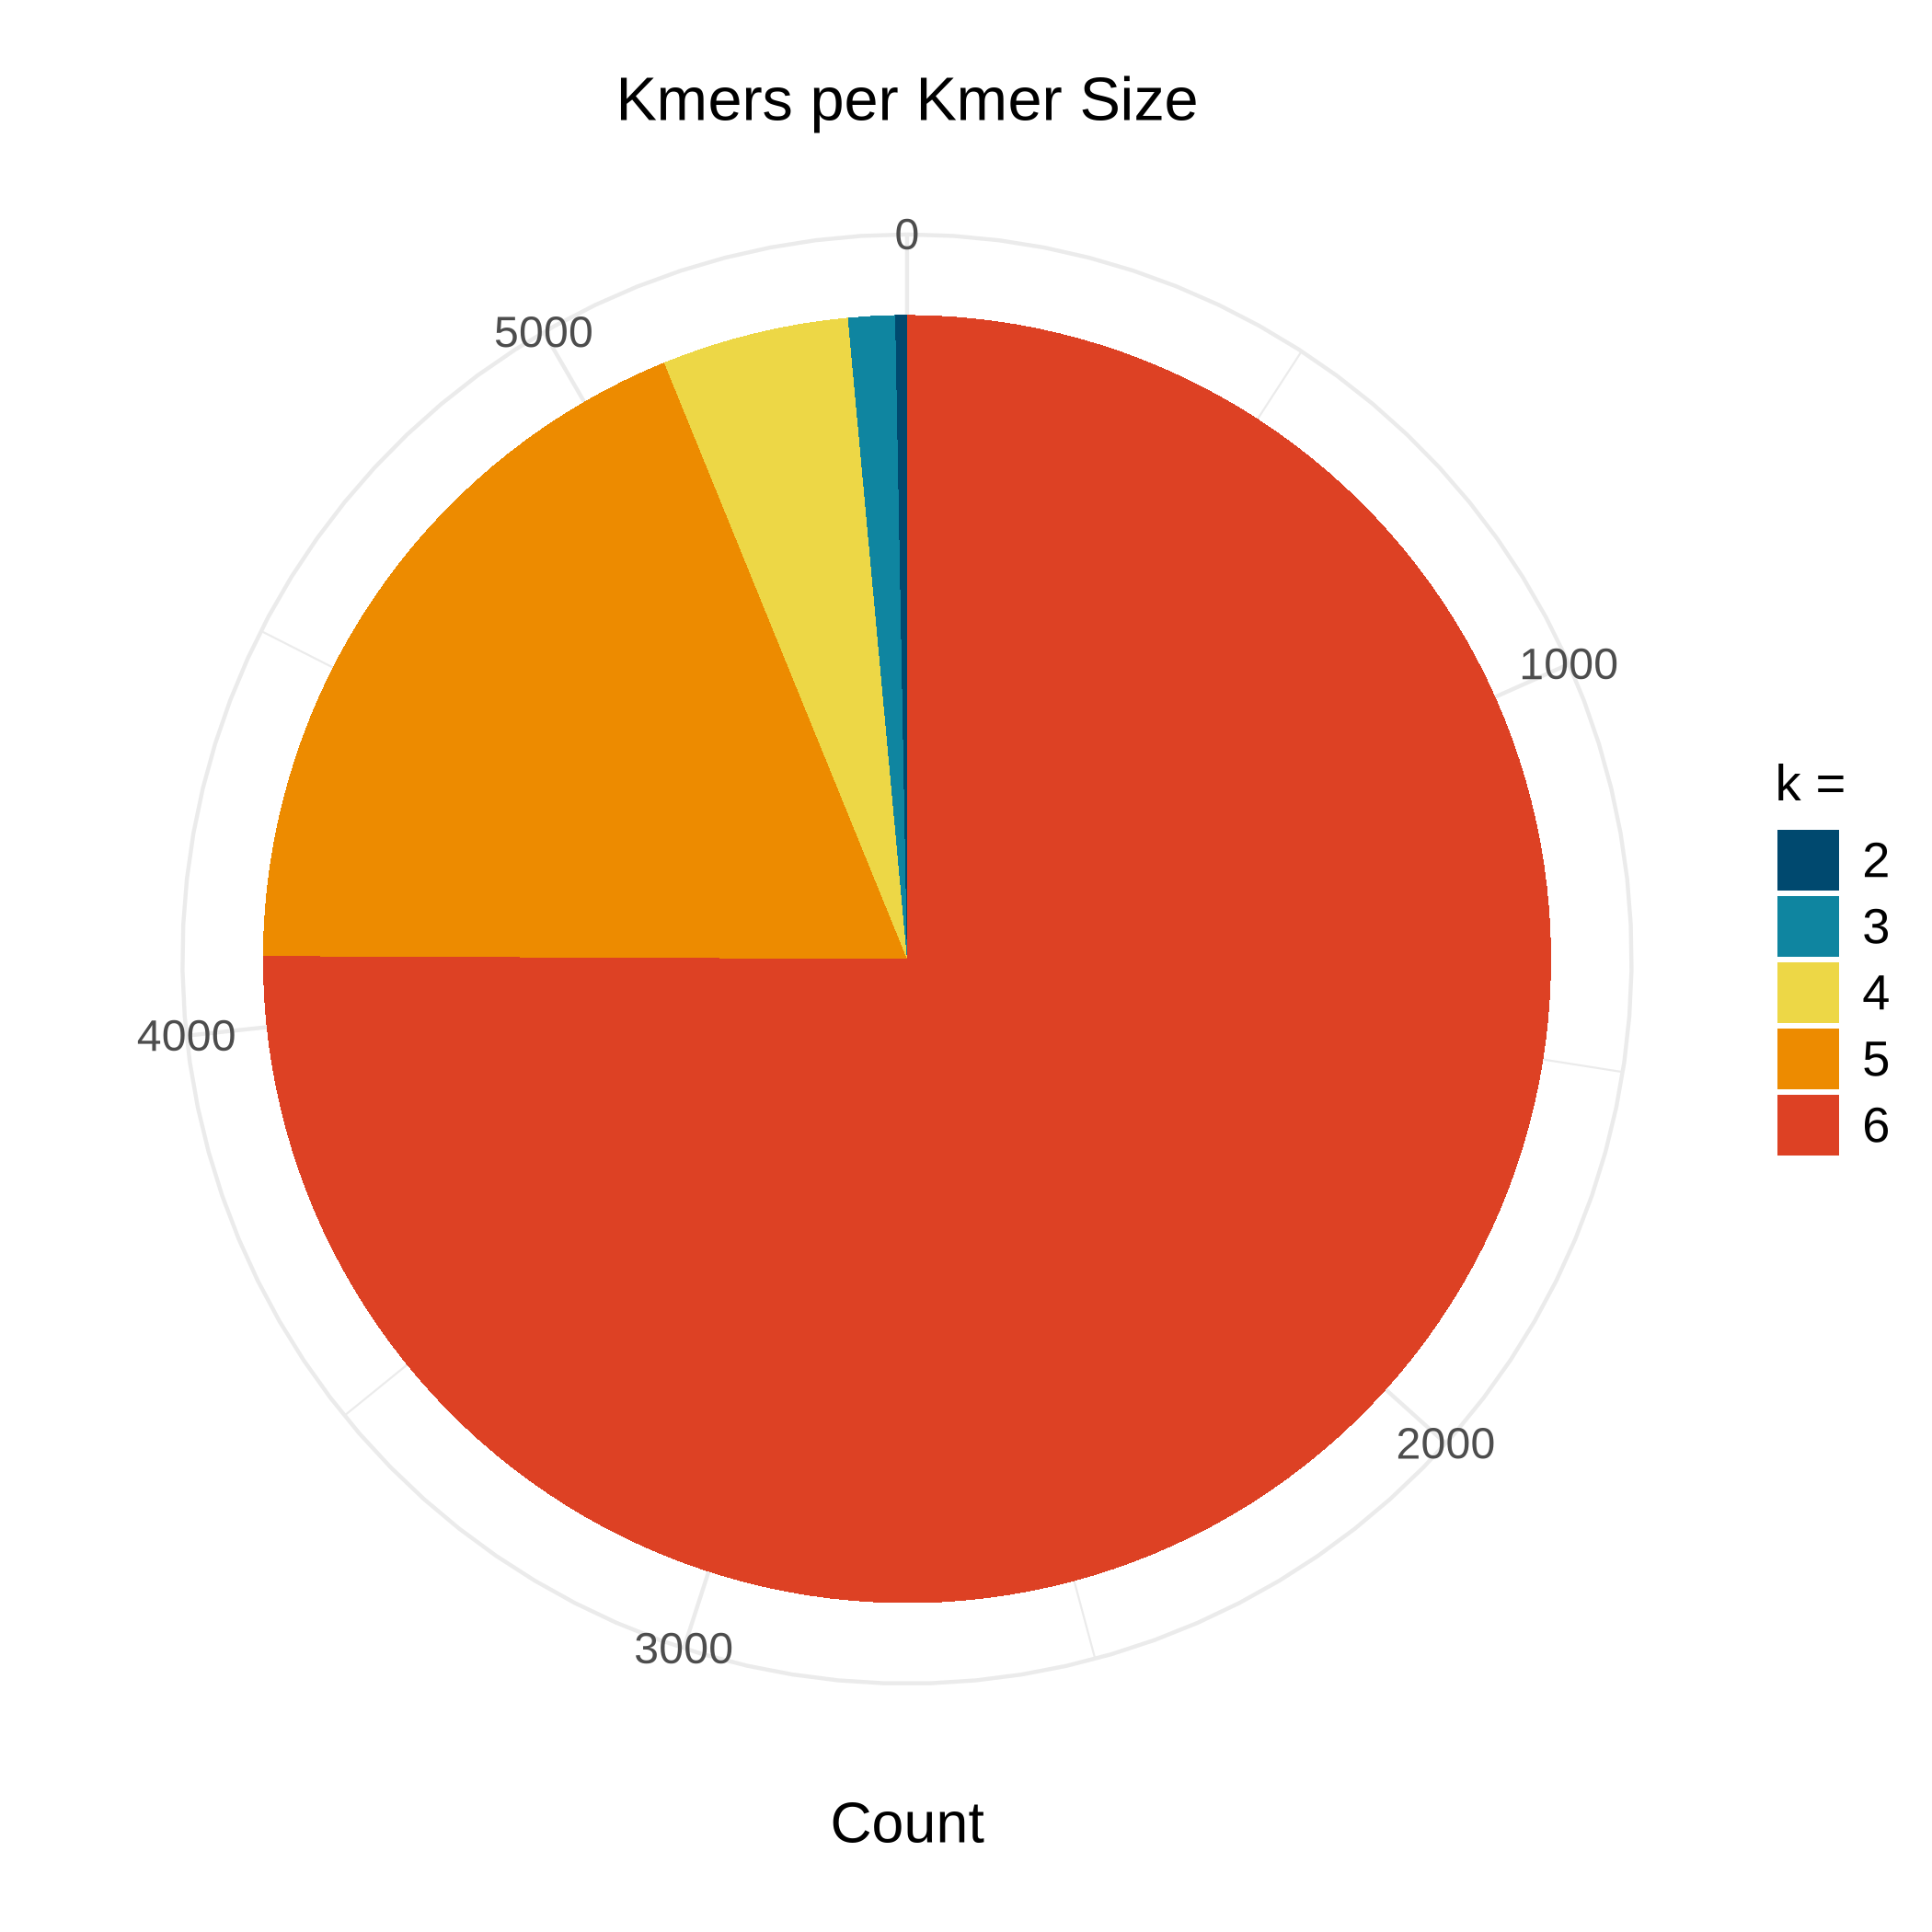
\includegraphics{gb-test-pdf_files/figure-pdf/kmer-set-sizes-1.png}
\end{center}

\begin{Shaded}
\begin{Highlighting}[]
\NormalTok{pe\_arr }\OtherTok{\textless{}{-}} \ControlFlowTok{function}\NormalTok{(seq\_data)}
  \FunctionTok{return}\NormalTok{(}\FunctionTok{array}\NormalTok{(seq\_data, }\AttributeTok{dim =} \FunctionTok{c}\NormalTok{((ldf}\DecValTok{{-}6}\NormalTok{)}\SpecialCharTok{/}\DecValTok{4}\NormalTok{, }\DecValTok{2}\NormalTok{),}
    \AttributeTok{dimnames =} \FunctionTok{list}\NormalTok{(}\DecValTok{1}\SpecialCharTok{:}\NormalTok{((ldf}\DecValTok{{-}6}\NormalTok{)}\SpecialCharTok{/}\DecValTok{4}\NormalTok{), }\FunctionTok{c}\NormalTok{(}\StringTok{"prom"}\NormalTok{,}\StringTok{"enha"}\NormalTok{))))}

\NormalTok{indxs }\OtherTok{\textless{}{-}} \FunctionTok{list}\NormalTok{(}
  \AttributeTok{prod =} \FunctionTok{pe\_arr}\NormalTok{(}\FunctionTok{c}\NormalTok{(}\FunctionTok{seq}\NormalTok{(}\DecValTok{7}\NormalTok{,ldf}\DecValTok{{-}3}\NormalTok{,}\DecValTok{4}\NormalTok{), ldf }\SpecialCharTok{+} \FunctionTok{seq}\NormalTok{(}\DecValTok{7}\NormalTok{,ldf}\DecValTok{{-}3}\NormalTok{,}\DecValTok{4}\NormalTok{))),}
  \AttributeTok{barc =} \FunctionTok{pe\_arr}\NormalTok{(}\FunctionTok{c}\NormalTok{(}\FunctionTok{seq}\NormalTok{(}\DecValTok{8}\NormalTok{,ldf}\DecValTok{{-}2}\NormalTok{,}\DecValTok{4}\NormalTok{), ldf }\SpecialCharTok{+} \FunctionTok{seq}\NormalTok{(}\DecValTok{8}\NormalTok{,ldf}\DecValTok{{-}2}\NormalTok{,}\DecValTok{4}\NormalTok{))),}
  \AttributeTok{pals =} \FunctionTok{pe\_arr}\NormalTok{(}\FunctionTok{c}\NormalTok{(}\FunctionTok{seq}\NormalTok{(}\DecValTok{9}\NormalTok{,ldf}\DecValTok{{-}1}\NormalTok{,}\DecValTok{4}\NormalTok{), ldf }\SpecialCharTok{+} \FunctionTok{seq}\NormalTok{(}\DecValTok{9}\NormalTok{,ldf}\DecValTok{{-}1}\NormalTok{,}\DecValTok{4}\NormalTok{))),}
  \AttributeTok{revc =} \FunctionTok{pe\_arr}\NormalTok{(}\FunctionTok{c}\NormalTok{(}\FunctionTok{seq}\NormalTok{(}\DecValTok{10}\NormalTok{,ldf,}\DecValTok{4}\NormalTok{), ldf }\SpecialCharTok{+} \FunctionTok{seq}\NormalTok{(}\DecValTok{10}\NormalTok{,ldf,}\DecValTok{4}\NormalTok{))))}
\end{Highlighting}
\end{Shaded}

Now, for the sake of text-space optimization, we'll make some plotting
functions (principally pyramid, bar and violin plots), in order to
visualize our data.

\begin{Shaded}
\begin{Highlighting}[]
\CommentTok{\# To plot pyramid{-}plots}
\NormalTok{pyrplot\_ }\OtherTok{\textless{}{-}} \ControlFlowTok{function}\NormalTok{(cre\_data, kmer\_labels, title, }
\NormalTok{                    x\_label, y\_label, y\_breaks) \{}
\NormalTok{  CREs }\OtherTok{\textless{}{-}} \FunctionTok{c}\NormalTok{(}\StringTok{"Enhancer"}\NormalTok{, }\StringTok{"Promoter"}\NormalTok{)}
\NormalTok{  field\_order }\OtherTok{\textless{}{-}} \FunctionTok{filter}\NormalTok{(cre\_data, Type}\SpecialCharTok{==}\NormalTok{CREs[}\DecValTok{1}\NormalTok{])}\SpecialCharTok{$}\NormalTok{Field}
\NormalTok{  fact\_field\_order }\OtherTok{\textless{}{-}} \FunctionTok{factor}\NormalTok{(cre\_data}\SpecialCharTok{$}\NormalTok{Field, field\_order)}

  \ControlFlowTok{if}\NormalTok{ (}\FunctionTok{missing}\NormalTok{(kmer\_labels)) kmer\_labels }\OtherTok{\textless{}{-}}\NormalTok{ field\_order}

  \FunctionTok{ggplot}\NormalTok{(cre\_data) }\SpecialCharTok{+}
    \FunctionTok{geom\_bar}\NormalTok{(}\FunctionTok{aes}\NormalTok{(}\AttributeTok{x =}\NormalTok{ fact\_field\_order, }
                 \AttributeTok{y =} \FunctionTok{ifelse}\NormalTok{(Type }\SpecialCharTok{==}\NormalTok{ CREs[}\DecValTok{1}\NormalTok{],}
                            \SpecialCharTok{{-}}\NormalTok{Means, Means), }
                 \AttributeTok{fill =} \FunctionTok{paste}\NormalTok{(Type, }\StringTok{"Means"}\NormalTok{)),}
             \AttributeTok{stat =} \StringTok{"identity"}\NormalTok{, }\AttributeTok{position =} \StringTok{"identity"}\NormalTok{, }
             \AttributeTok{alpha =} \FloatTok{0.6}\NormalTok{, }\AttributeTok{width =} \FloatTok{0.7}\NormalTok{) }\SpecialCharTok{+}
    \FunctionTok{geom\_errorbar}\NormalTok{(}\FunctionTok{aes}\NormalTok{(}\AttributeTok{x =}\NormalTok{ fact\_field\_order,}
                      \AttributeTok{ymin =} \FunctionTok{ifelse}\NormalTok{(Type }\SpecialCharTok{==}\NormalTok{ CREs[}\DecValTok{1}\NormalTok{],}
                                   \SpecialCharTok{{-}}\NormalTok{Means }\SpecialCharTok{+}\NormalTok{ StDevs,}
\NormalTok{                                    Means }\SpecialCharTok{{-}}\NormalTok{ StDevs),}
                      \AttributeTok{ymax =} \FunctionTok{ifelse}\NormalTok{(Type }\SpecialCharTok{==}\NormalTok{ CREs[}\DecValTok{1}\NormalTok{],}
                                   \SpecialCharTok{{-}}\NormalTok{Means }\SpecialCharTok{{-}}\NormalTok{ StDevs,}
\NormalTok{                                    Means }\SpecialCharTok{+}\NormalTok{ StDevs)),}
                  \AttributeTok{width =} \FloatTok{0.5}\NormalTok{, }\AttributeTok{alpha =} \FloatTok{0.6}\NormalTok{,}
                  \AttributeTok{colour =} \StringTok{"black"}\NormalTok{) }\SpecialCharTok{+}
    \FunctionTok{coord\_flip}\NormalTok{() }\SpecialCharTok{+}
    \FunctionTok{scale\_x\_discrete}\NormalTok{(}\AttributeTok{labels =}\NormalTok{ kmer\_labels) }\SpecialCharTok{+}
    \FunctionTok{scale\_y\_continuous}\NormalTok{(}\AttributeTok{breaks =}\NormalTok{ y\_breaks,}
                       \AttributeTok{labels =} \FunctionTok{abs}\NormalTok{(y\_breaks)) }\SpecialCharTok{+}
    \FunctionTok{scale\_fill\_manual}\NormalTok{(}\AttributeTok{values =} \FunctionTok{c}\NormalTok{(}\StringTok{"turquoise"}\NormalTok{, }\StringTok{"coral"}\NormalTok{),}
                      \AttributeTok{labels =}\NormalTok{ CREs) }\SpecialCharTok{+}
    \FunctionTok{labs}\NormalTok{(}\AttributeTok{y =} \StringTok{"Means"}\NormalTok{, }\AttributeTok{x =}\NormalTok{ x\_label,}
         \AttributeTok{title =}\NormalTok{ title, }\AttributeTok{fill =} \StringTok{"CRE Type"}\NormalTok{) }\SpecialCharTok{+}
    \FunctionTok{theme\_minimal}\NormalTok{() }\SpecialCharTok{+}
    \FunctionTok{theme}\NormalTok{(}\AttributeTok{legend.position =} \StringTok{"bottom"}\NormalTok{,}
          \AttributeTok{axis.title =} \FunctionTok{element\_text}\NormalTok{(}\AttributeTok{size =} \DecValTok{15}\NormalTok{),}
          \AttributeTok{text =} \FunctionTok{element\_text}\NormalTok{(}\AttributeTok{size =} \FunctionTok{rel}\NormalTok{(}\FloatTok{4.25}\NormalTok{)),}
          \AttributeTok{legend.text =} \FunctionTok{element\_text}\NormalTok{(}\AttributeTok{size =} \DecValTok{13}\NormalTok{),}
          \AttributeTok{legend.title =} \FunctionTok{element\_text}\NormalTok{(}\AttributeTok{size =} \FloatTok{13.5}\NormalTok{),}
          \AttributeTok{axis.text.y =} \FunctionTok{element\_text}\NormalTok{(}\AttributeTok{family =} \StringTok{"mono"}\NormalTok{),}
          \AttributeTok{plot.title =} \FunctionTok{element\_text}\NormalTok{(}\AttributeTok{size =} \DecValTok{16}\NormalTok{, }\AttributeTok{hjust =} \FloatTok{0.5}\NormalTok{))}
\NormalTok{\}}

\NormalTok{barplot\_ }\OtherTok{\textless{}{-}} \ControlFlowTok{function}\NormalTok{(cre\_data, y\_breaks, }\AttributeTok{y\_axis\_title=}\StringTok{""}\NormalTok{,}
                     \AttributeTok{fill\_legend\_title=}\StringTok{""}\NormalTok{) \{}
  \FunctionTok{ggplot}\NormalTok{(cre\_data) }\SpecialCharTok{+}
    \FunctionTok{geom\_bar}\NormalTok{(}\FunctionTok{aes}\NormalTok{(}\AttributeTok{x =} \FunctionTok{factor}\NormalTok{(Type), }
                 \AttributeTok{y =}\NormalTok{ Means, }\AttributeTok{fill =}\NormalTok{ Type),}
             \AttributeTok{stat =} \StringTok{"identity"}\NormalTok{, }\AttributeTok{position =} \StringTok{"identity"}\NormalTok{,}
             \AttributeTok{alpha =} \FloatTok{0.6}\NormalTok{) }\SpecialCharTok{+}
    \FunctionTok{geom\_errorbar}\NormalTok{(}\FunctionTok{aes}\NormalTok{(}\AttributeTok{x =} \FunctionTok{factor}\NormalTok{(Type), }
                      \AttributeTok{ymin =}\NormalTok{ Means }\SpecialCharTok{{-}}\NormalTok{ StDevs,}
                      \AttributeTok{ymax =}\NormalTok{ Means }\SpecialCharTok{+}\NormalTok{ StDevs),}
                  \AttributeTok{alpha =} \FloatTok{0.6}\NormalTok{, }\AttributeTok{width =} \FloatTok{0.5}\NormalTok{,}
                  \AttributeTok{colour =} \StringTok{"black"}\NormalTok{) }\SpecialCharTok{+}
    \FunctionTok{labs}\NormalTok{(}\AttributeTok{y =}\NormalTok{ y\_axis\_title, }\AttributeTok{x =} \StringTok{""}\NormalTok{,}
         \AttributeTok{fill =}\NormalTok{ fill\_legend\_title) }\SpecialCharTok{+}
    \FunctionTok{scale\_y\_continuous}\NormalTok{(}\AttributeTok{breaks =}\NormalTok{ y\_breaks,}
                       \AttributeTok{labels =}\NormalTok{ y\_breaks) }\SpecialCharTok{+}
    \FunctionTok{scale\_fill\_manual}\NormalTok{(}\AttributeTok{values =} \FunctionTok{c}\NormalTok{(}\StringTok{"turquoise"}\NormalTok{, }\StringTok{"coral"}\NormalTok{)) }\SpecialCharTok{+}
    \FunctionTok{theme\_minimal}\NormalTok{() }\SpecialCharTok{+}
    \FunctionTok{theme}\NormalTok{(}\AttributeTok{legend.position =} \StringTok{"none"}\NormalTok{,}
          \AttributeTok{text =} \FunctionTok{element\_text}\NormalTok{(}\AttributeTok{size =} \FunctionTok{rel}\NormalTok{(}\FloatTok{4.5}\NormalTok{)),}
          \AttributeTok{axis.title =} \FunctionTok{element\_text}\NormalTok{(}\AttributeTok{size =} \DecValTok{16}\NormalTok{))}
\NormalTok{\}}

\NormalTok{hvioplot\_ }\OtherTok{\textless{}{-}} \ControlFlowTok{function}\NormalTok{(data, y\_var, }\AttributeTok{y\_label =} \StringTok{""}\NormalTok{,}
                     \AttributeTok{fill\_legend\_title =} \StringTok{""}\NormalTok{) \{}
  \CommentTok{\# x\_breaks \textless{}{-} seq({-}0.12,0.12,0.06)}
  \FunctionTok{ggplot}\NormalTok{(data, }\FunctionTok{aes}\NormalTok{(}\AttributeTok{x =} \DecValTok{0}\NormalTok{, }\AttributeTok{y =} \SpecialCharTok{!!}\FunctionTok{sym}\NormalTok{(y\_var), }\AttributeTok{fill =}\NormalTok{ type)) }\SpecialCharTok{+}
    \FunctionTok{geom\_violinhalf}\NormalTok{(}\AttributeTok{flip =} \DecValTok{1}\NormalTok{, }\AttributeTok{adjust =} \FloatTok{0.25}\NormalTok{,}
                    \AttributeTok{trim =} \ConstantTok{FALSE}\NormalTok{, }\AttributeTok{scale =} \StringTok{"count"}\NormalTok{,}
                    \AttributeTok{position =} \FunctionTok{position\_dodge}\NormalTok{(}\AttributeTok{width =} \DecValTok{0}\NormalTok{),}
                    \AttributeTok{linewidth =} \FloatTok{0.1}\NormalTok{, }\AttributeTok{alpha =} \FloatTok{0.6}\NormalTok{) }\SpecialCharTok{+}
    \FunctionTok{theme\_minimal}\NormalTok{() }\SpecialCharTok{+}
    \CommentTok{\# scale\_x\_continuous(breaks = x\_breaks ,}
    \CommentTok{\#                    labels = abs(x\_breaks )) +}
    \FunctionTok{scale\_fill\_manual}\NormalTok{(}\AttributeTok{values =} \FunctionTok{c}\NormalTok{(}\StringTok{"turquoise"}\NormalTok{, }\StringTok{"coral"}\NormalTok{)) }\SpecialCharTok{+}
    \FunctionTok{labs}\NormalTok{(}\AttributeTok{x =} \StringTok{""}\NormalTok{, }\AttributeTok{y =}\NormalTok{ y\_label, }\AttributeTok{fill =}\NormalTok{ fill\_legend\_title) }\SpecialCharTok{+}
    \FunctionTok{theme}\NormalTok{(}\AttributeTok{legend.position =} \StringTok{"none"}\NormalTok{,}
          \AttributeTok{text =} \FunctionTok{element\_text}\NormalTok{(}\AttributeTok{size =} \FunctionTok{rel}\NormalTok{(}\FloatTok{4.5}\NormalTok{)),}
          \AttributeTok{axis.title =} \FunctionTok{element\_text}\NormalTok{(}\AttributeTok{size =} \DecValTok{13}\NormalTok{))}
\NormalTok{\}}
\end{Highlighting}
\end{Shaded}

\begin{Shaded}
\begin{Highlighting}[]
\FunctionTok{pyrplot\_}\NormalTok{(cre\_summary[}\FunctionTok{c}\NormalTok{(}\DecValTok{1}\SpecialCharTok{:}\DecValTok{4}\NormalTok{, ldf }\SpecialCharTok{+}\NormalTok{ (}\DecValTok{1}\SpecialCharTok{:}\DecValTok{4}\NormalTok{)), ], }
      \AttributeTok{x\_label =} \StringTok{"Nucleotides"}\NormalTok{, }\AttributeTok{y\_breaks =} \FunctionTok{seq}\NormalTok{(}\SpecialCharTok{{-}}\DecValTok{1}\NormalTok{,}\DecValTok{1}\NormalTok{,}\FloatTok{0.2}\NormalTok{), }
      \AttributeTok{title =} \StringTok{"Percentage Means per Nucleotide"}\NormalTok{)}
\end{Highlighting}
\end{Shaded}

\begin{center}
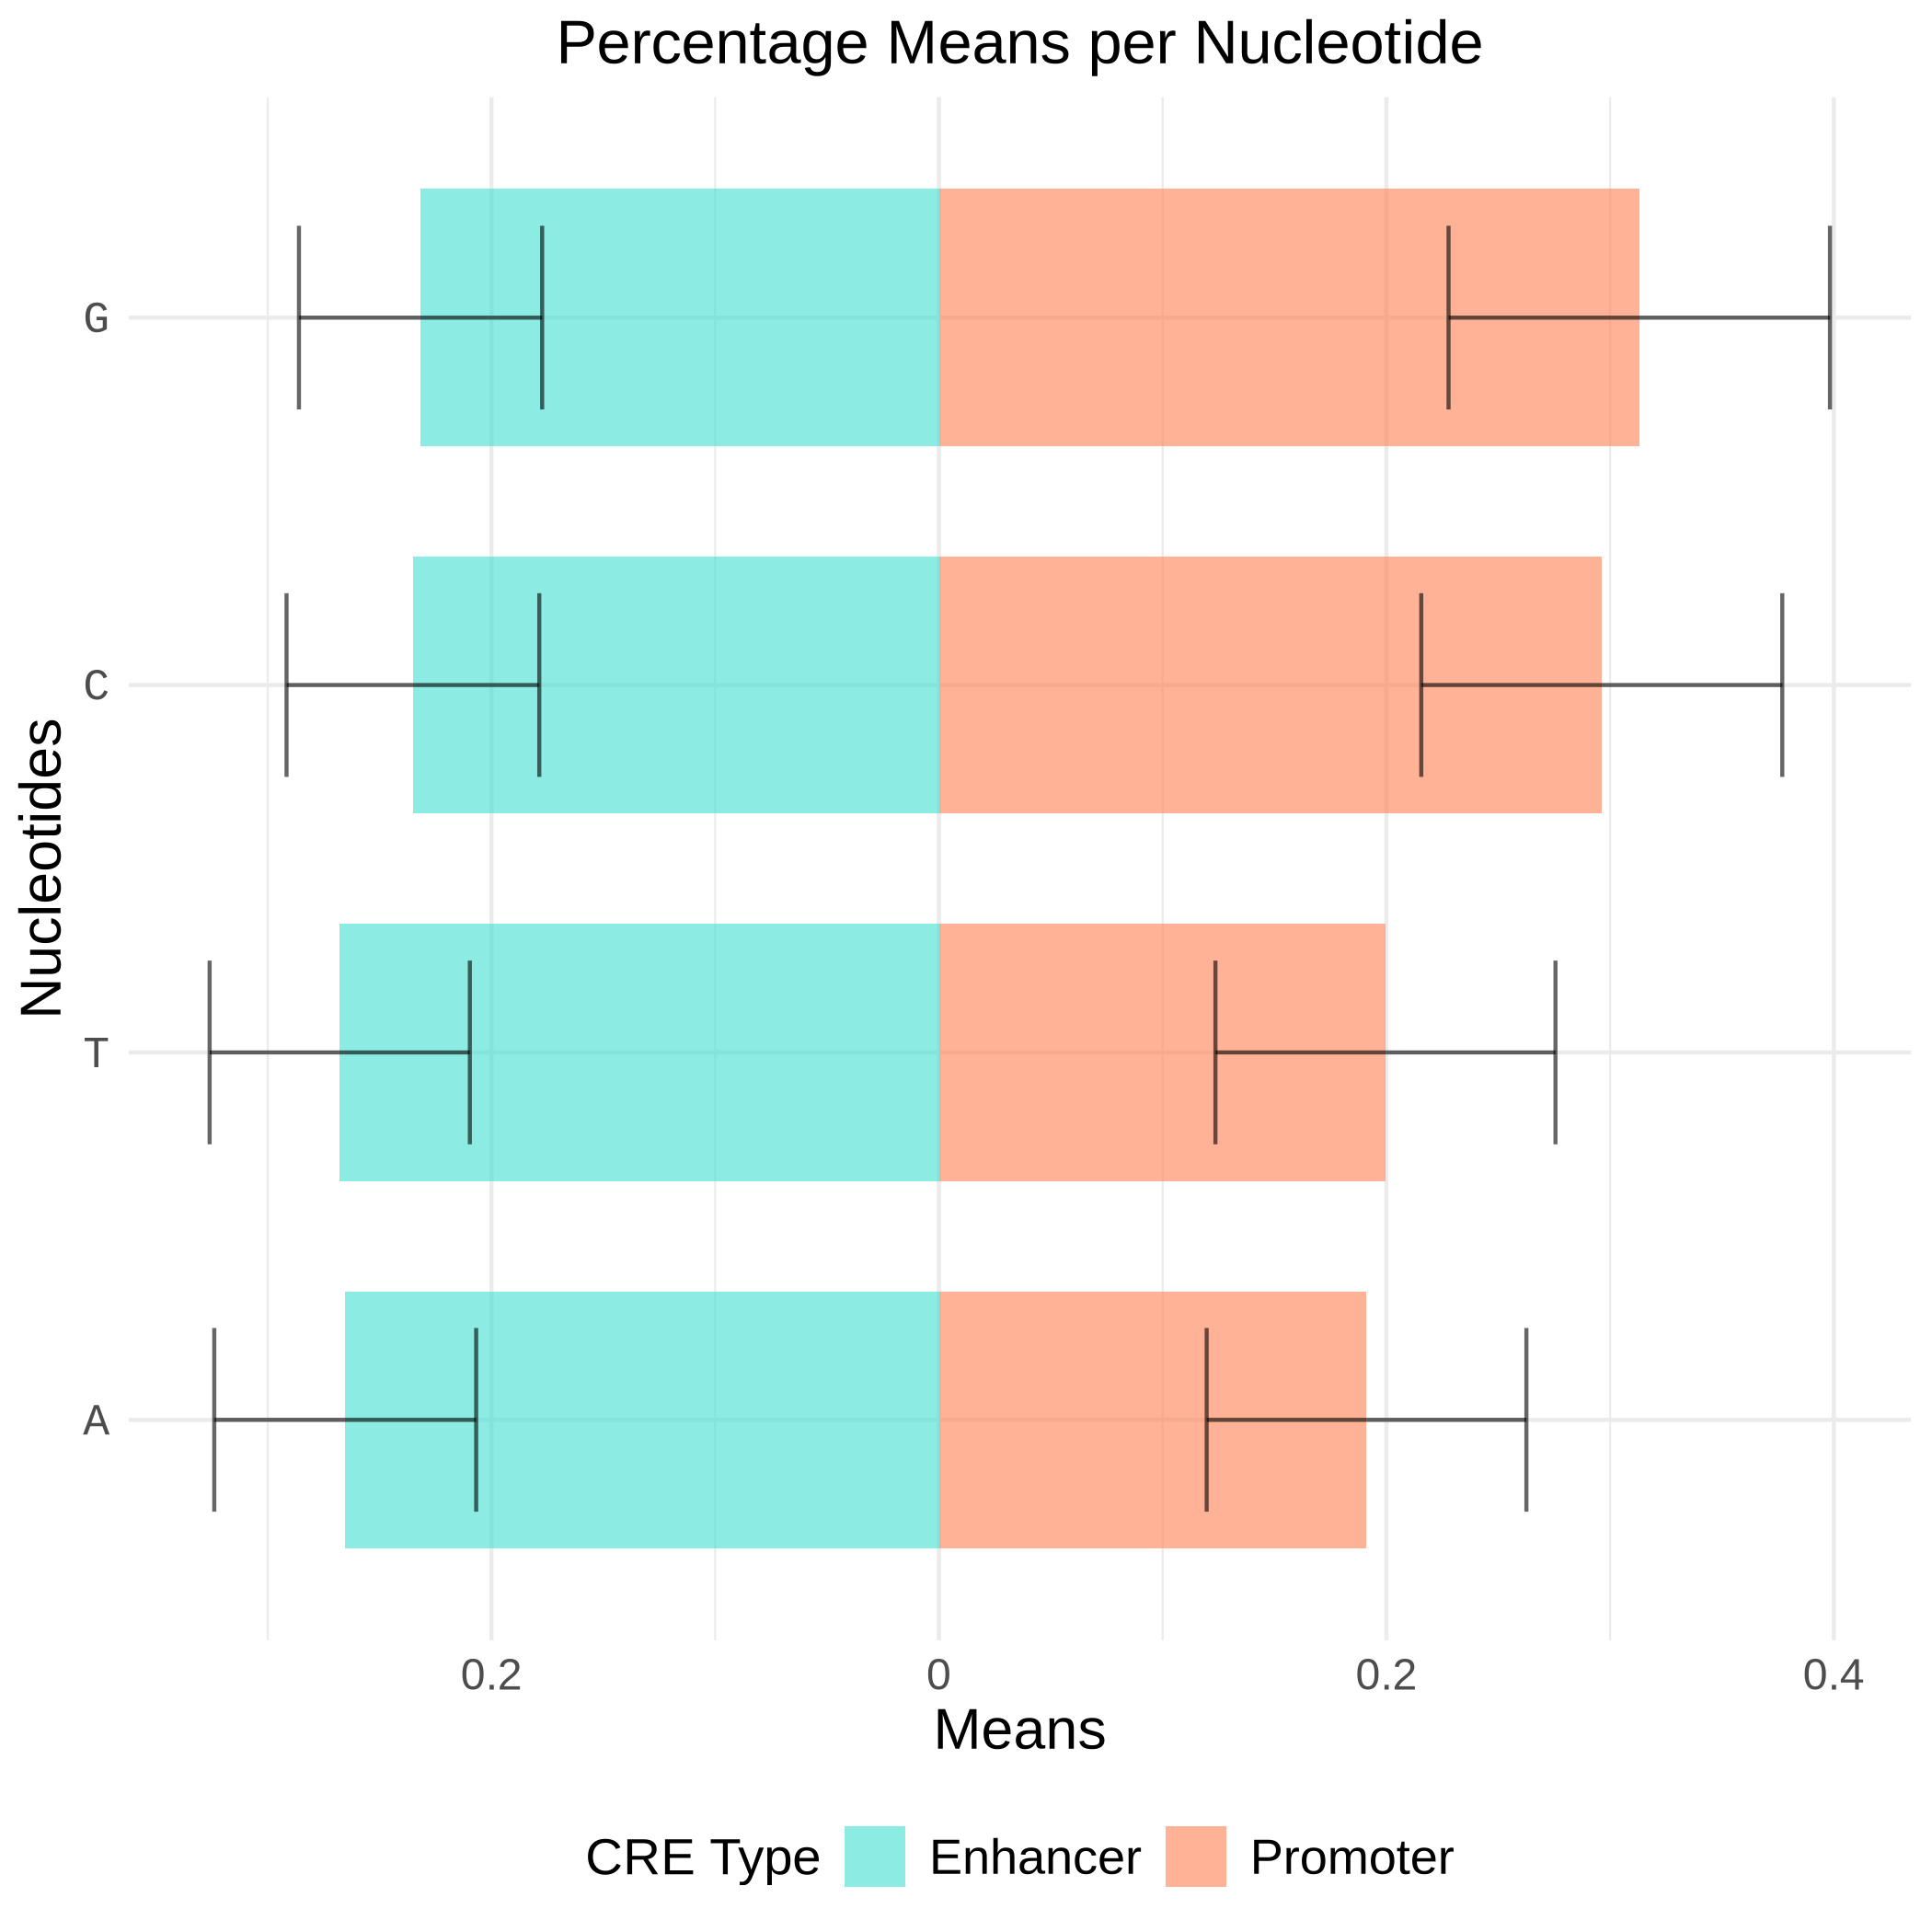
\includegraphics{gb-test-pdf_files/figure-pdf/figure-nucl-1.png}
\end{center}

\begin{Shaded}
\begin{Highlighting}[]
\NormalTok{data\_e }\OtherTok{\textless{}{-}} \FunctionTok{cbind}\NormalTok{(}\AttributeTok{type =} \FunctionTok{rep}\NormalTok{(}\StringTok{"Enhancer"}\NormalTok{,}
                \FunctionTok{length}\NormalTok{(enhas}\SpecialCharTok{$}\NormalTok{temp)), enhas[,}\DecValTok{5}\SpecialCharTok{:}\DecValTok{6}\NormalTok{])}
\NormalTok{data\_p }\OtherTok{\textless{}{-}} \FunctionTok{cbind}\NormalTok{(}\AttributeTok{type =} \FunctionTok{rep}\NormalTok{(}\StringTok{"Promoter"}\NormalTok{,}
                \FunctionTok{length}\NormalTok{(proms}\SpecialCharTok{$}\NormalTok{temp)), proms[,}\DecValTok{5}\SpecialCharTok{:}\DecValTok{6}\NormalTok{])}
\NormalTok{subset\_tm\_sh }\OtherTok{\textless{}{-}} \FunctionTok{rbind}\NormalTok{(data\_e, data\_p)}
\end{Highlighting}
\end{Shaded}

\begin{Shaded}
\begin{Highlighting}[]
\CommentTok{\# Saving Melting Temperature Violin Plot }
\NormalTok{tm\_violin }\OtherTok{\textless{}{-}} \FunctionTok{hvioplot\_}\NormalTok{(}\AttributeTok{data =}\NormalTok{ subset\_tm\_sh, }
                       \AttributeTok{y\_var =} \StringTok{"temp"}\NormalTok{, }
                       \AttributeTok{y\_label =} \StringTok{"Density"}\NormalTok{)}

\CommentTok{\# Saving Shannon Violin Plot }
\NormalTok{sh\_violin }\OtherTok{\textless{}{-}} \FunctionTok{hvioplot\_}\NormalTok{(}\AttributeTok{data =}\NormalTok{ subset\_tm\_sh, }
                       \AttributeTok{y\_var =} \StringTok{"shan"}\NormalTok{, }
                       \AttributeTok{fill\_legend\_title =} \StringTok{"CRE Type"}\NormalTok{)}

\CommentTok{\# Get legend}
\NormalTok{legend\_violin }\OtherTok{\textless{}{-}} \FunctionTok{get\_legend\_bypass}\NormalTok{(sh\_violin }\SpecialCharTok{+}
  \FunctionTok{guides}\NormalTok{(}\AttributeTok{color =} \FunctionTok{guide\_legend}\NormalTok{(}\AttributeTok{nrow =} \DecValTok{1}\NormalTok{)) }\SpecialCharTok{+}
  \FunctionTok{theme}\NormalTok{(}\AttributeTok{legend.position =} \StringTok{"bottom"}\NormalTok{,}
        \AttributeTok{legend.title =} \FunctionTok{element\_text}\NormalTok{(}\AttributeTok{size =} \FloatTok{13.5}\NormalTok{),}
        \AttributeTok{legend.text =} \FunctionTok{element\_text}\NormalTok{(}\AttributeTok{size =} \DecValTok{13}\NormalTok{)))}

\CommentTok{\# Merging of Violin{-}Plots }
\NormalTok{grid\_violin }\OtherTok{\textless{}{-}} \FunctionTok{plot\_grid}\NormalTok{(tm\_violin, sh\_violin, }\ConstantTok{NULL}\NormalTok{,}
                 \AttributeTok{ncol =} \DecValTok{3}\NormalTok{, }\AttributeTok{rel\_widths =} \FunctionTok{c}\NormalTok{(}\DecValTok{1}\NormalTok{,}\DecValTok{1}\NormalTok{,}\FloatTok{0.1}\NormalTok{),}
                 \AttributeTok{labels =} \FunctionTok{c}\NormalTok{(}\StringTok{"Melting Temperature"}\NormalTok{,}
                 \StringTok{"Shannon Entropy"}\NormalTok{), }\AttributeTok{label\_size =} \DecValTok{16}\NormalTok{,}
                 \AttributeTok{label\_fontface =} \StringTok{"plain"}\NormalTok{, }\AttributeTok{vjust =} \DecValTok{1}\NormalTok{,}
                 \AttributeTok{hjust =} \FunctionTok{c}\NormalTok{(}\SpecialCharTok{{-}}\FloatTok{0.38}\NormalTok{, }\SpecialCharTok{{-}}\FloatTok{0.48}\NormalTok{))}

\CommentTok{\# Adding legend at the bottom}
\FunctionTok{plot\_grid}\NormalTok{(grid\_violin, legend\_violin,}
          \AttributeTok{ncol =} \DecValTok{1}\NormalTok{, }\AttributeTok{rel\_heights =} \FunctionTok{c}\NormalTok{(}\DecValTok{12}\NormalTok{,}\DecValTok{1}\NormalTok{))}
\end{Highlighting}
\end{Shaded}

\begin{center}
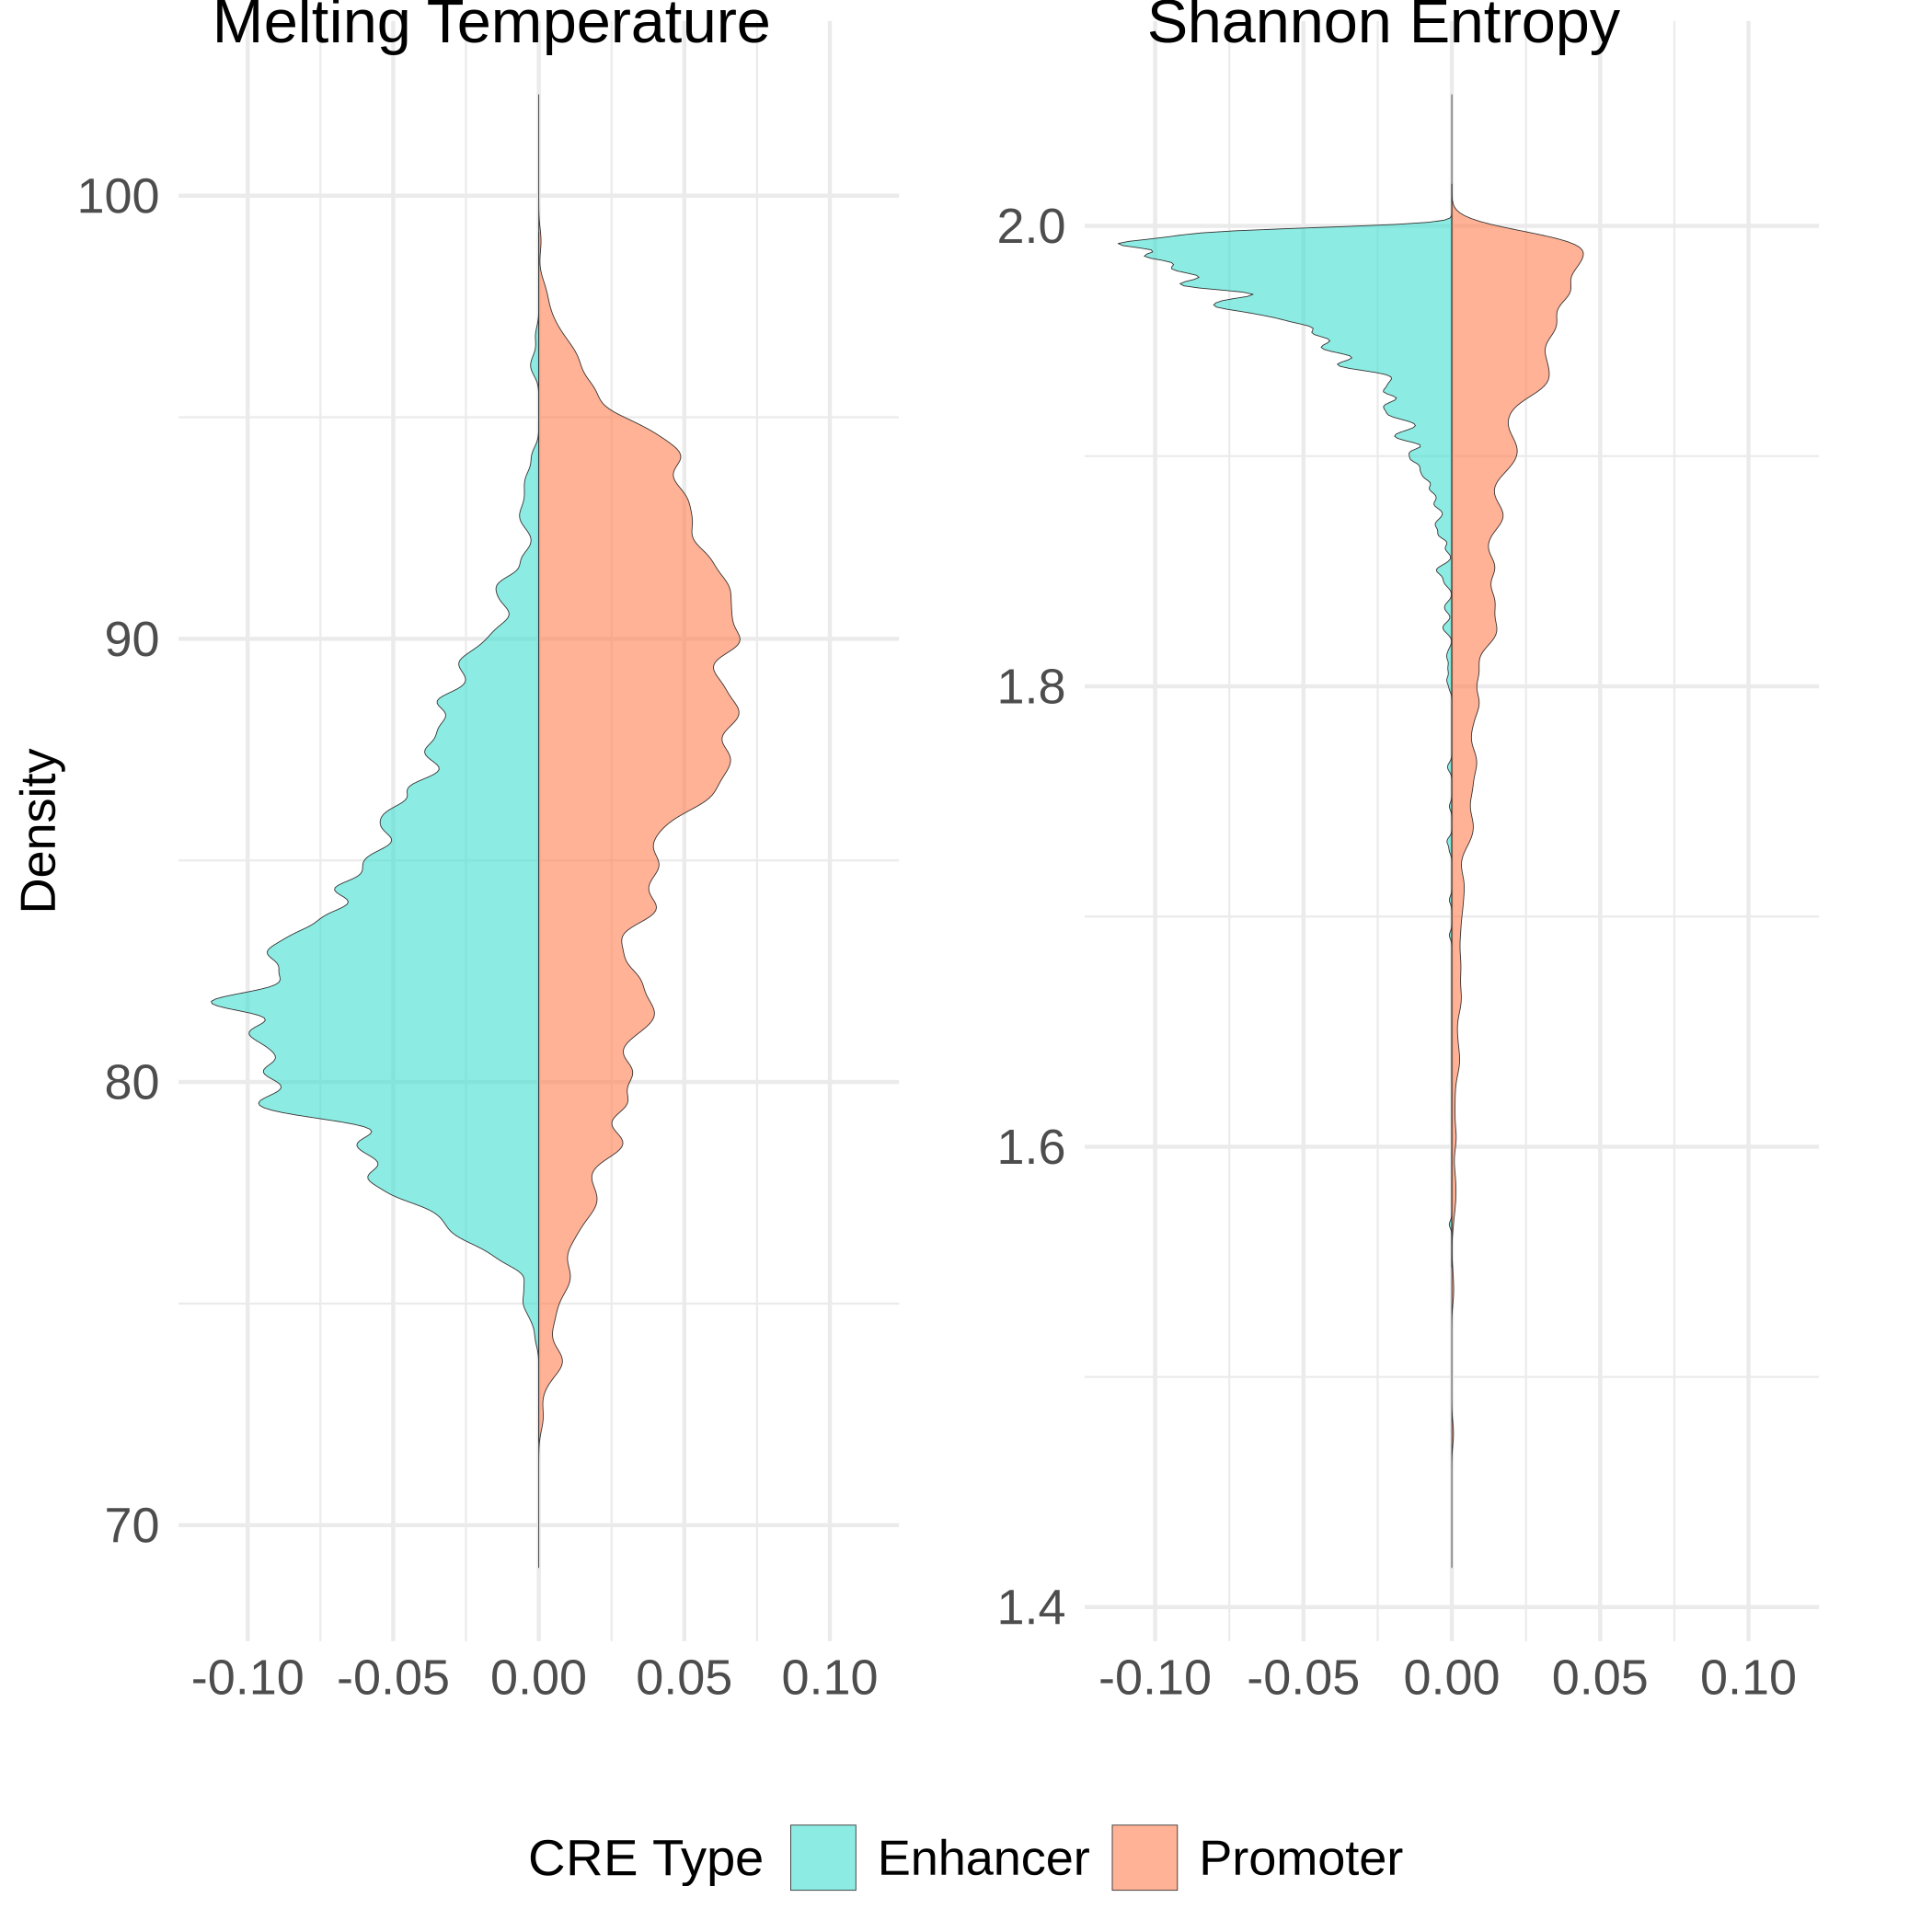
\includegraphics{gb-test-pdf_files/figure-pdf/subset-temp-shan-3-1.png}
\end{center}

\begin{Shaded}
\begin{Highlighting}[]
\CommentTok{\# Saving Melting Temperature Bar{-}Plot}
\NormalTok{temp\_plot }\OtherTok{\textless{}{-}} \FunctionTok{barplot\_}\NormalTok{(}\FunctionTok{filter}\NormalTok{(cre\_summary, Field}\SpecialCharTok{==}\StringTok{"temp"}\NormalTok{), }
                      \AttributeTok{y\_breaks =} \FunctionTok{seq}\NormalTok{(}\DecValTok{0}\NormalTok{, }\DecValTok{100}\NormalTok{, }\DecValTok{10}\NormalTok{), }
                      \AttributeTok{y\_axis\_title =} \StringTok{"Means"}\NormalTok{)}

\CommentTok{\# Saving Shannon Coefficient Bar{-}Plot}
\NormalTok{shan\_plot }\OtherTok{\textless{}{-}} \FunctionTok{barplot\_}\NormalTok{(}\FunctionTok{filter}\NormalTok{(cre\_summary, Field}\SpecialCharTok{==}\StringTok{"shan"}\NormalTok{), }
                      \AttributeTok{y\_breaks =} \FunctionTok{seq}\NormalTok{(}\DecValTok{0}\NormalTok{, }\DecValTok{2}\NormalTok{, }\FloatTok{0.25}\NormalTok{), }
                      \AttributeTok{fill\_legend\_title =} \StringTok{"CRE Type"}\NormalTok{)}

\CommentTok{\# Merging of Bar{-}Plots}
\FunctionTok{plot\_grid}\NormalTok{(temp\_plot, shan\_plot,  }
    \AttributeTok{ncol =} \DecValTok{2}\NormalTok{, }\AttributeTok{rel\_widths =} \FunctionTok{c}\NormalTok{(}\DecValTok{1}\NormalTok{,}\DecValTok{1}\NormalTok{), }
    \AttributeTok{vjust =} \DecValTok{1}\NormalTok{, }\AttributeTok{hjust =} \FunctionTok{c}\NormalTok{(}\SpecialCharTok{{-}}\FloatTok{0.35}\NormalTok{, }\SpecialCharTok{{-}}\FloatTok{0.48}\NormalTok{),}
    \AttributeTok{label\_size =} \DecValTok{16}\NormalTok{, }\AttributeTok{label\_fontface =} \StringTok{"plain"}\NormalTok{,}
    \AttributeTok{labels =} \FunctionTok{c}\NormalTok{(}\StringTok{"Melting Temperature"}\NormalTok{, }\StringTok{"Shannon Entropy"}\NormalTok{)) }
\end{Highlighting}
\end{Shaded}

\begin{center}
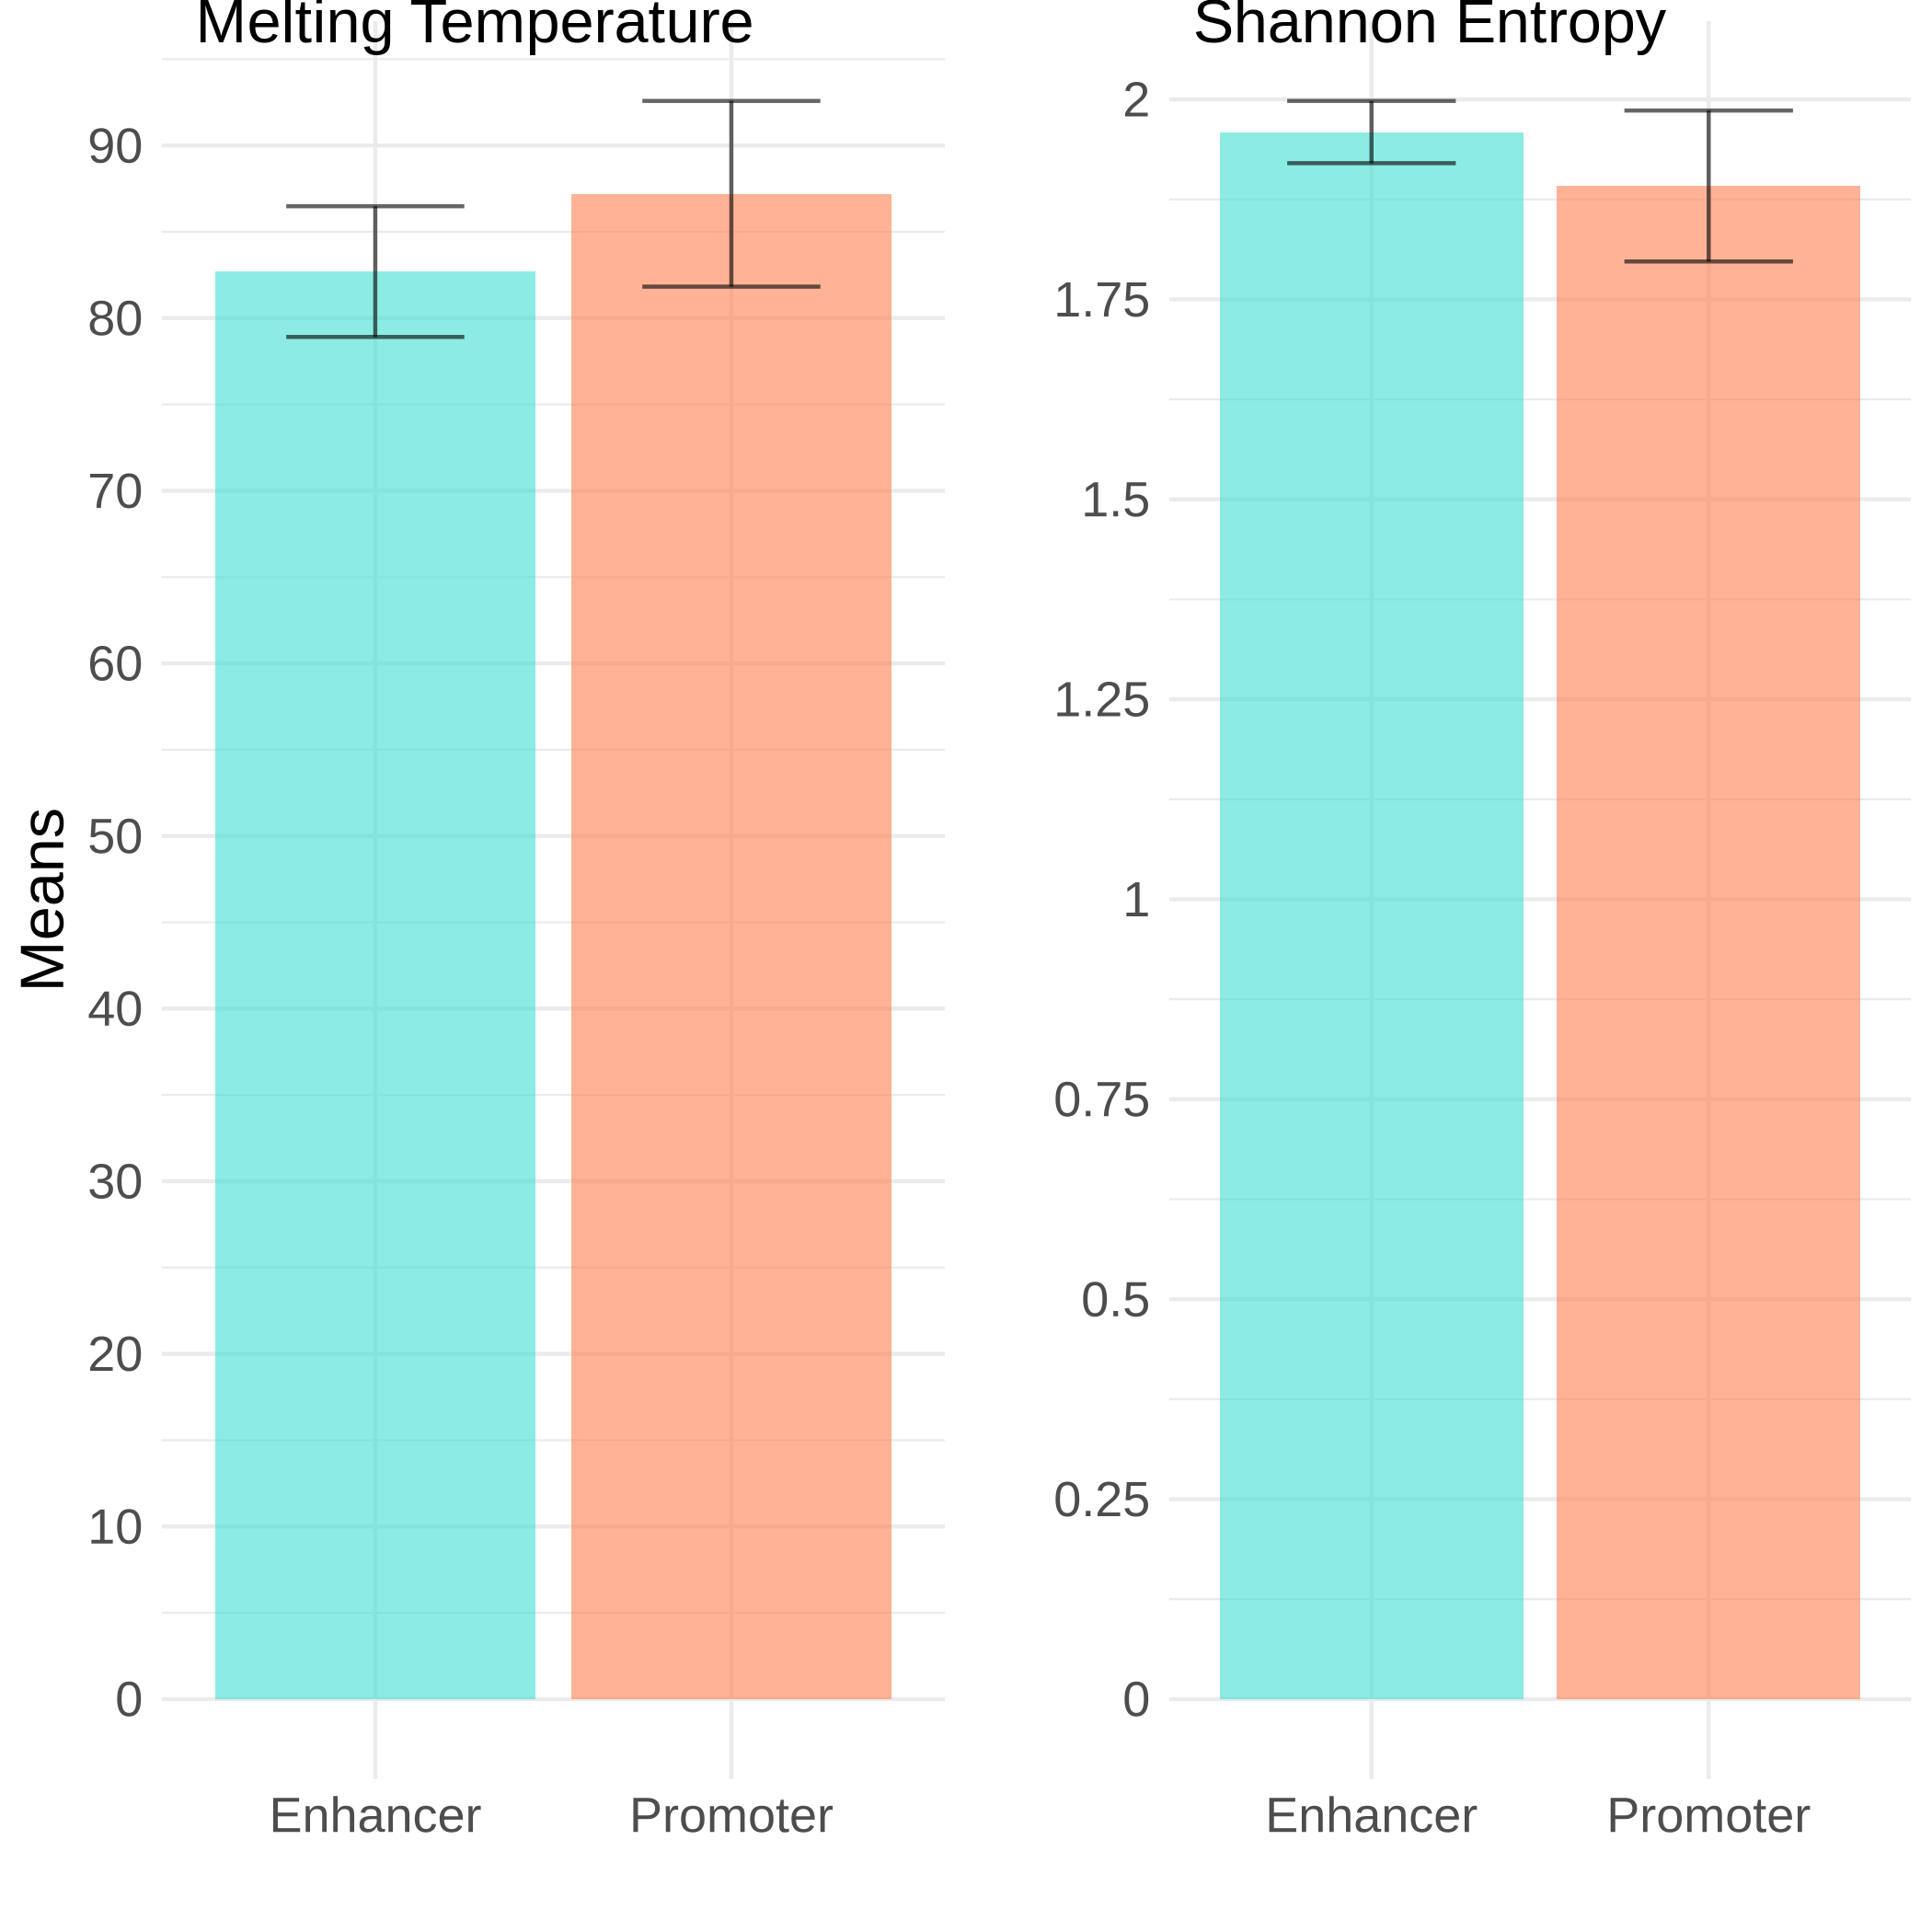
\includegraphics{gb-test-pdf_files/figure-pdf/figure-shan-temp-1.png}
\end{center}

\begin{Shaded}
\begin{Highlighting}[]
\NormalTok{kmer\_names }\OtherTok{\textless{}{-}} \FunctionTok{combi\_kmers}\NormalTok{(}\AttributeTok{k=}\DecValTok{3}\NormalTok{)[}\DecValTok{1}\SpecialCharTok{:}\DecValTok{48}\NormalTok{]}

\FunctionTok{pyrplot\_}\NormalTok{(cre\_summary[indxs}\SpecialCharTok{$}\NormalTok{prod[}\DecValTok{17}\SpecialCharTok{:}\DecValTok{64}\NormalTok{,],], kmer\_names,}
         \AttributeTok{x\_label =} \StringTok{"Kmers"}\NormalTok{, }\AttributeTok{y\_breaks =} \FunctionTok{seq}\NormalTok{(}\SpecialCharTok{{-}}\DecValTok{30}\NormalTok{,}\DecValTok{30}\NormalTok{,}\DecValTok{10}\NormalTok{), }
         \AttributeTok{title =} \StringTok{"KSG{-}Product Means per Kmer"}\NormalTok{)}
\end{Highlighting}
\end{Shaded}

\begin{center}
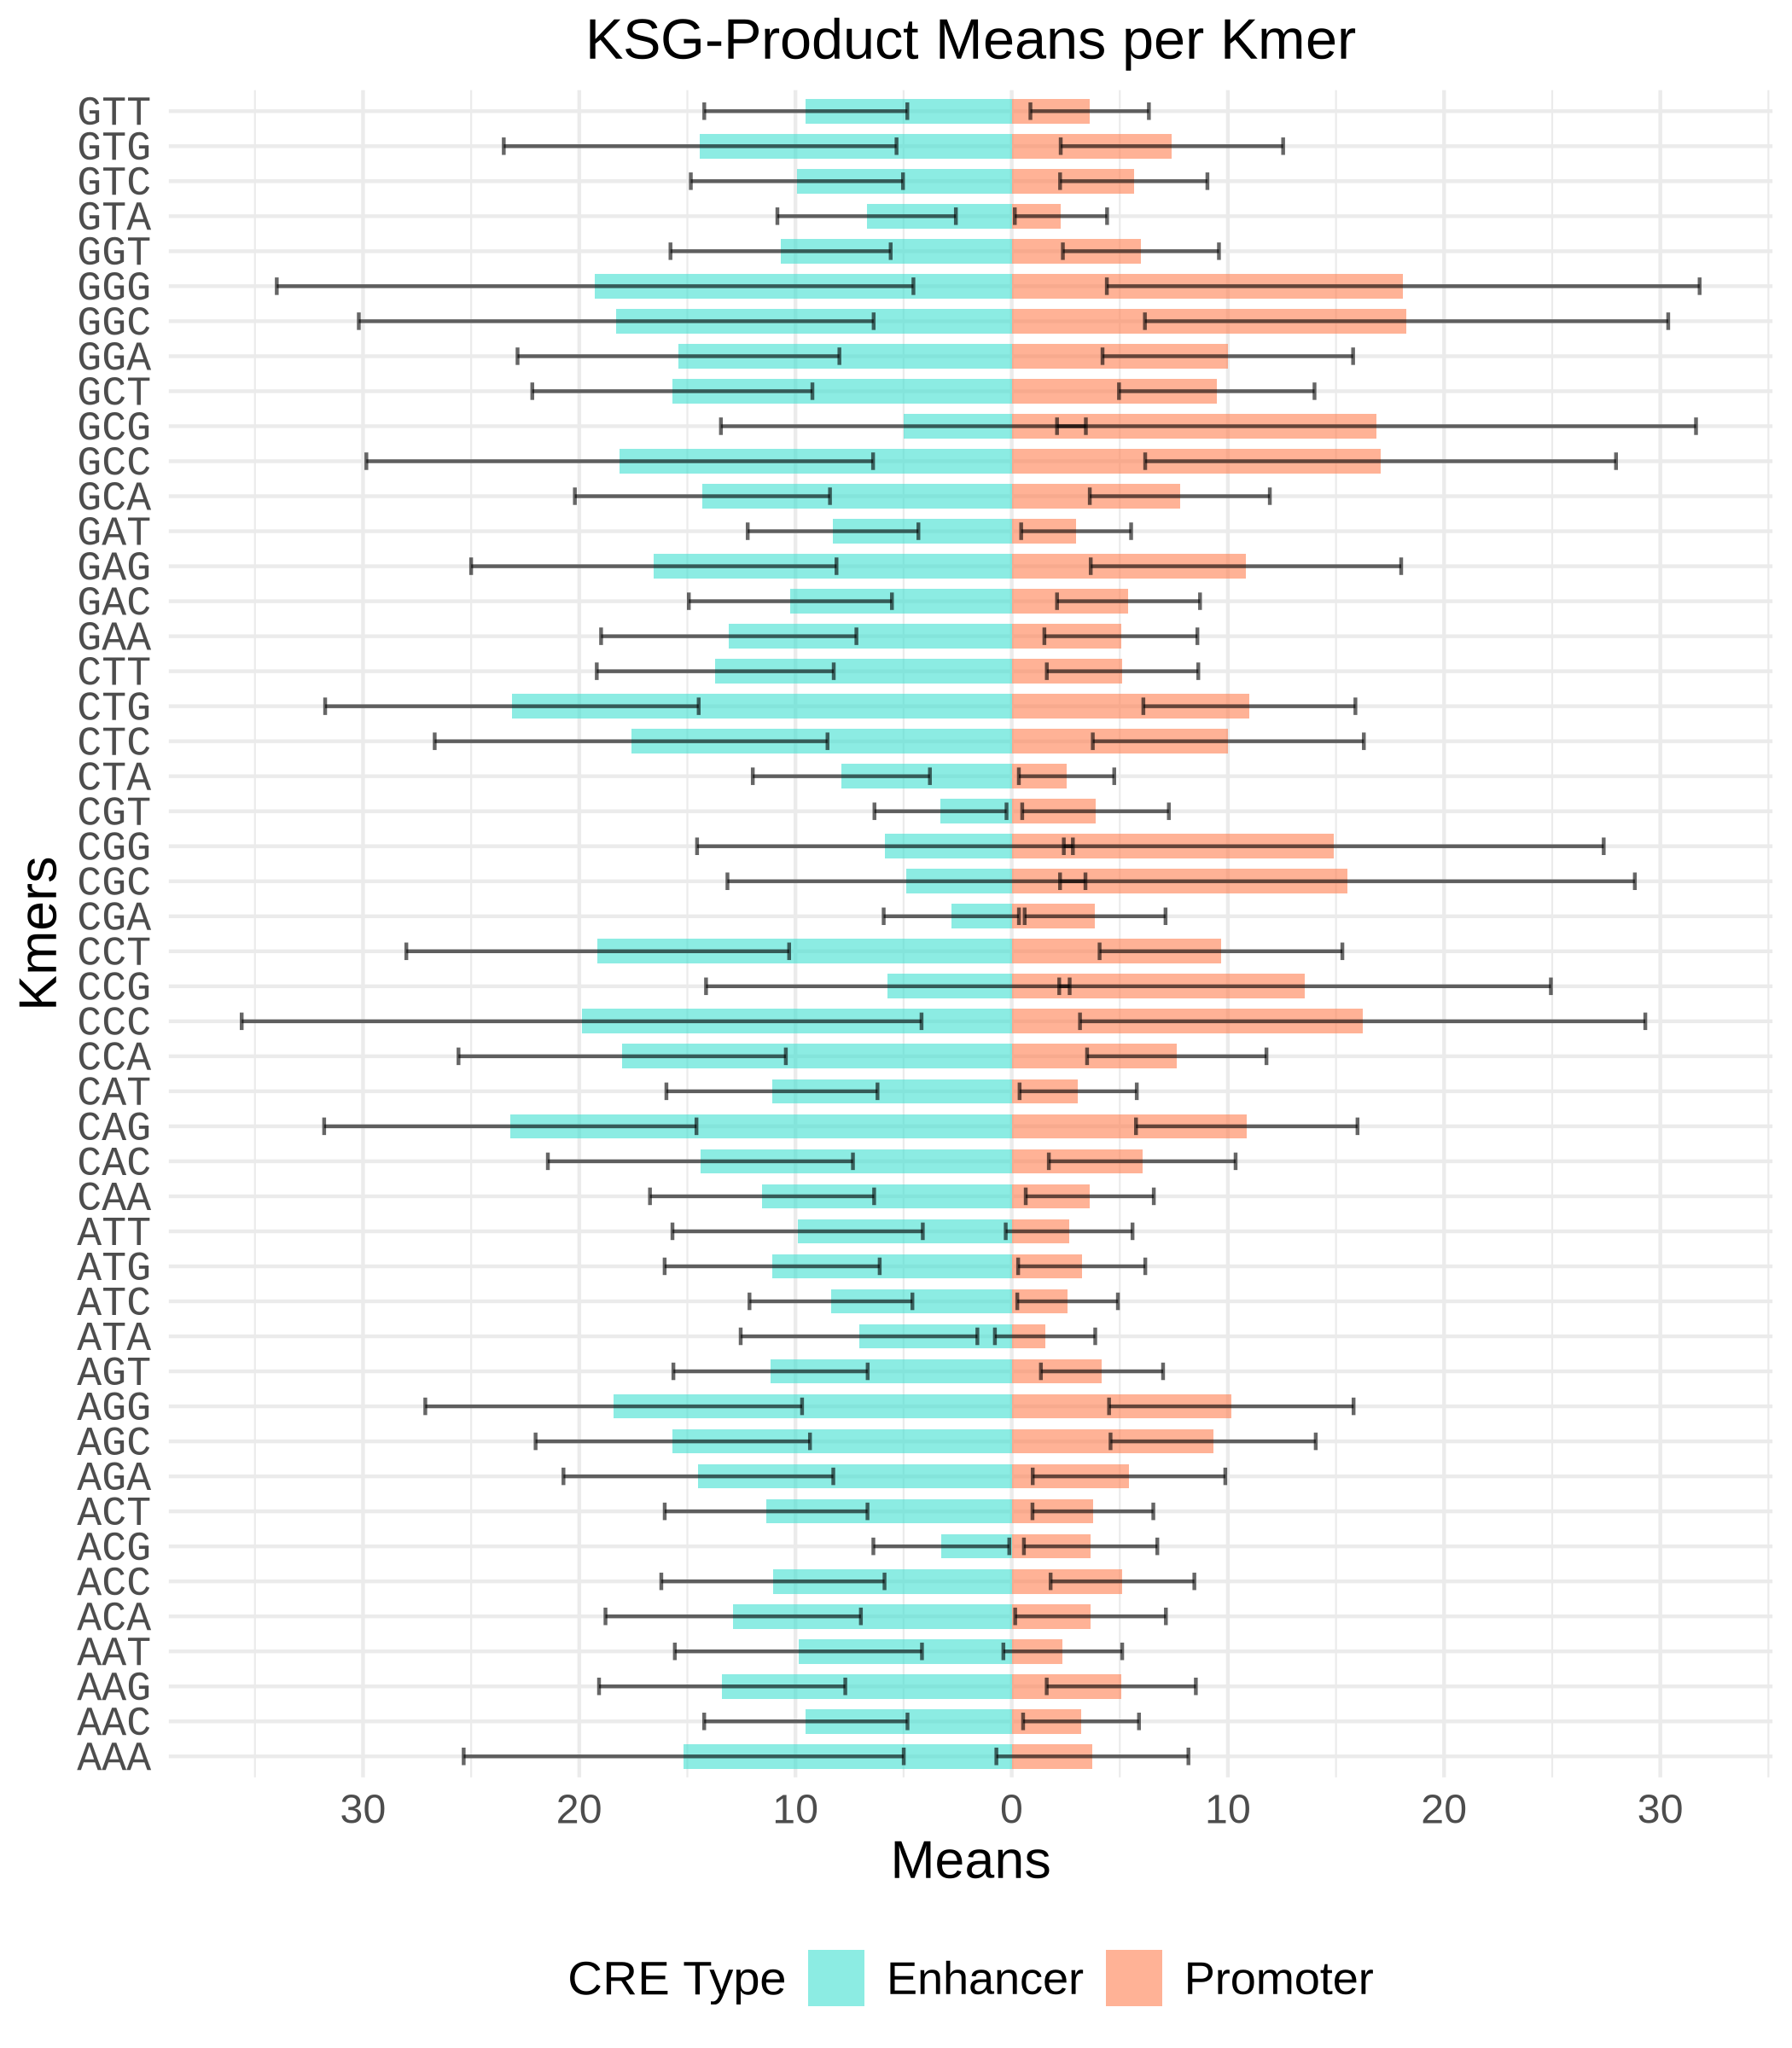
\includegraphics{gb-test-pdf_files/figure-pdf/figure-prods-1.png}
\end{center}

\begin{Shaded}
\begin{Highlighting}[]
\FunctionTok{pyrplot\_}\NormalTok{(cre\_summary[indxs}\SpecialCharTok{$}\NormalTok{barc[}\DecValTok{17}\SpecialCharTok{:}\DecValTok{64}\NormalTok{,],], kmer\_names,}
         \AttributeTok{x\_label =} \StringTok{"Kmers"}\NormalTok{, }\AttributeTok{y\_breaks =} \FunctionTok{seq}\NormalTok{(}\SpecialCharTok{{-}}\DecValTok{10}\NormalTok{,}\DecValTok{10}\NormalTok{,}\DecValTok{1}\NormalTok{), }
         \AttributeTok{title =} \StringTok{"Barcode Profile Means per Kmer"}\NormalTok{)}
\end{Highlighting}
\end{Shaded}

\begin{center}
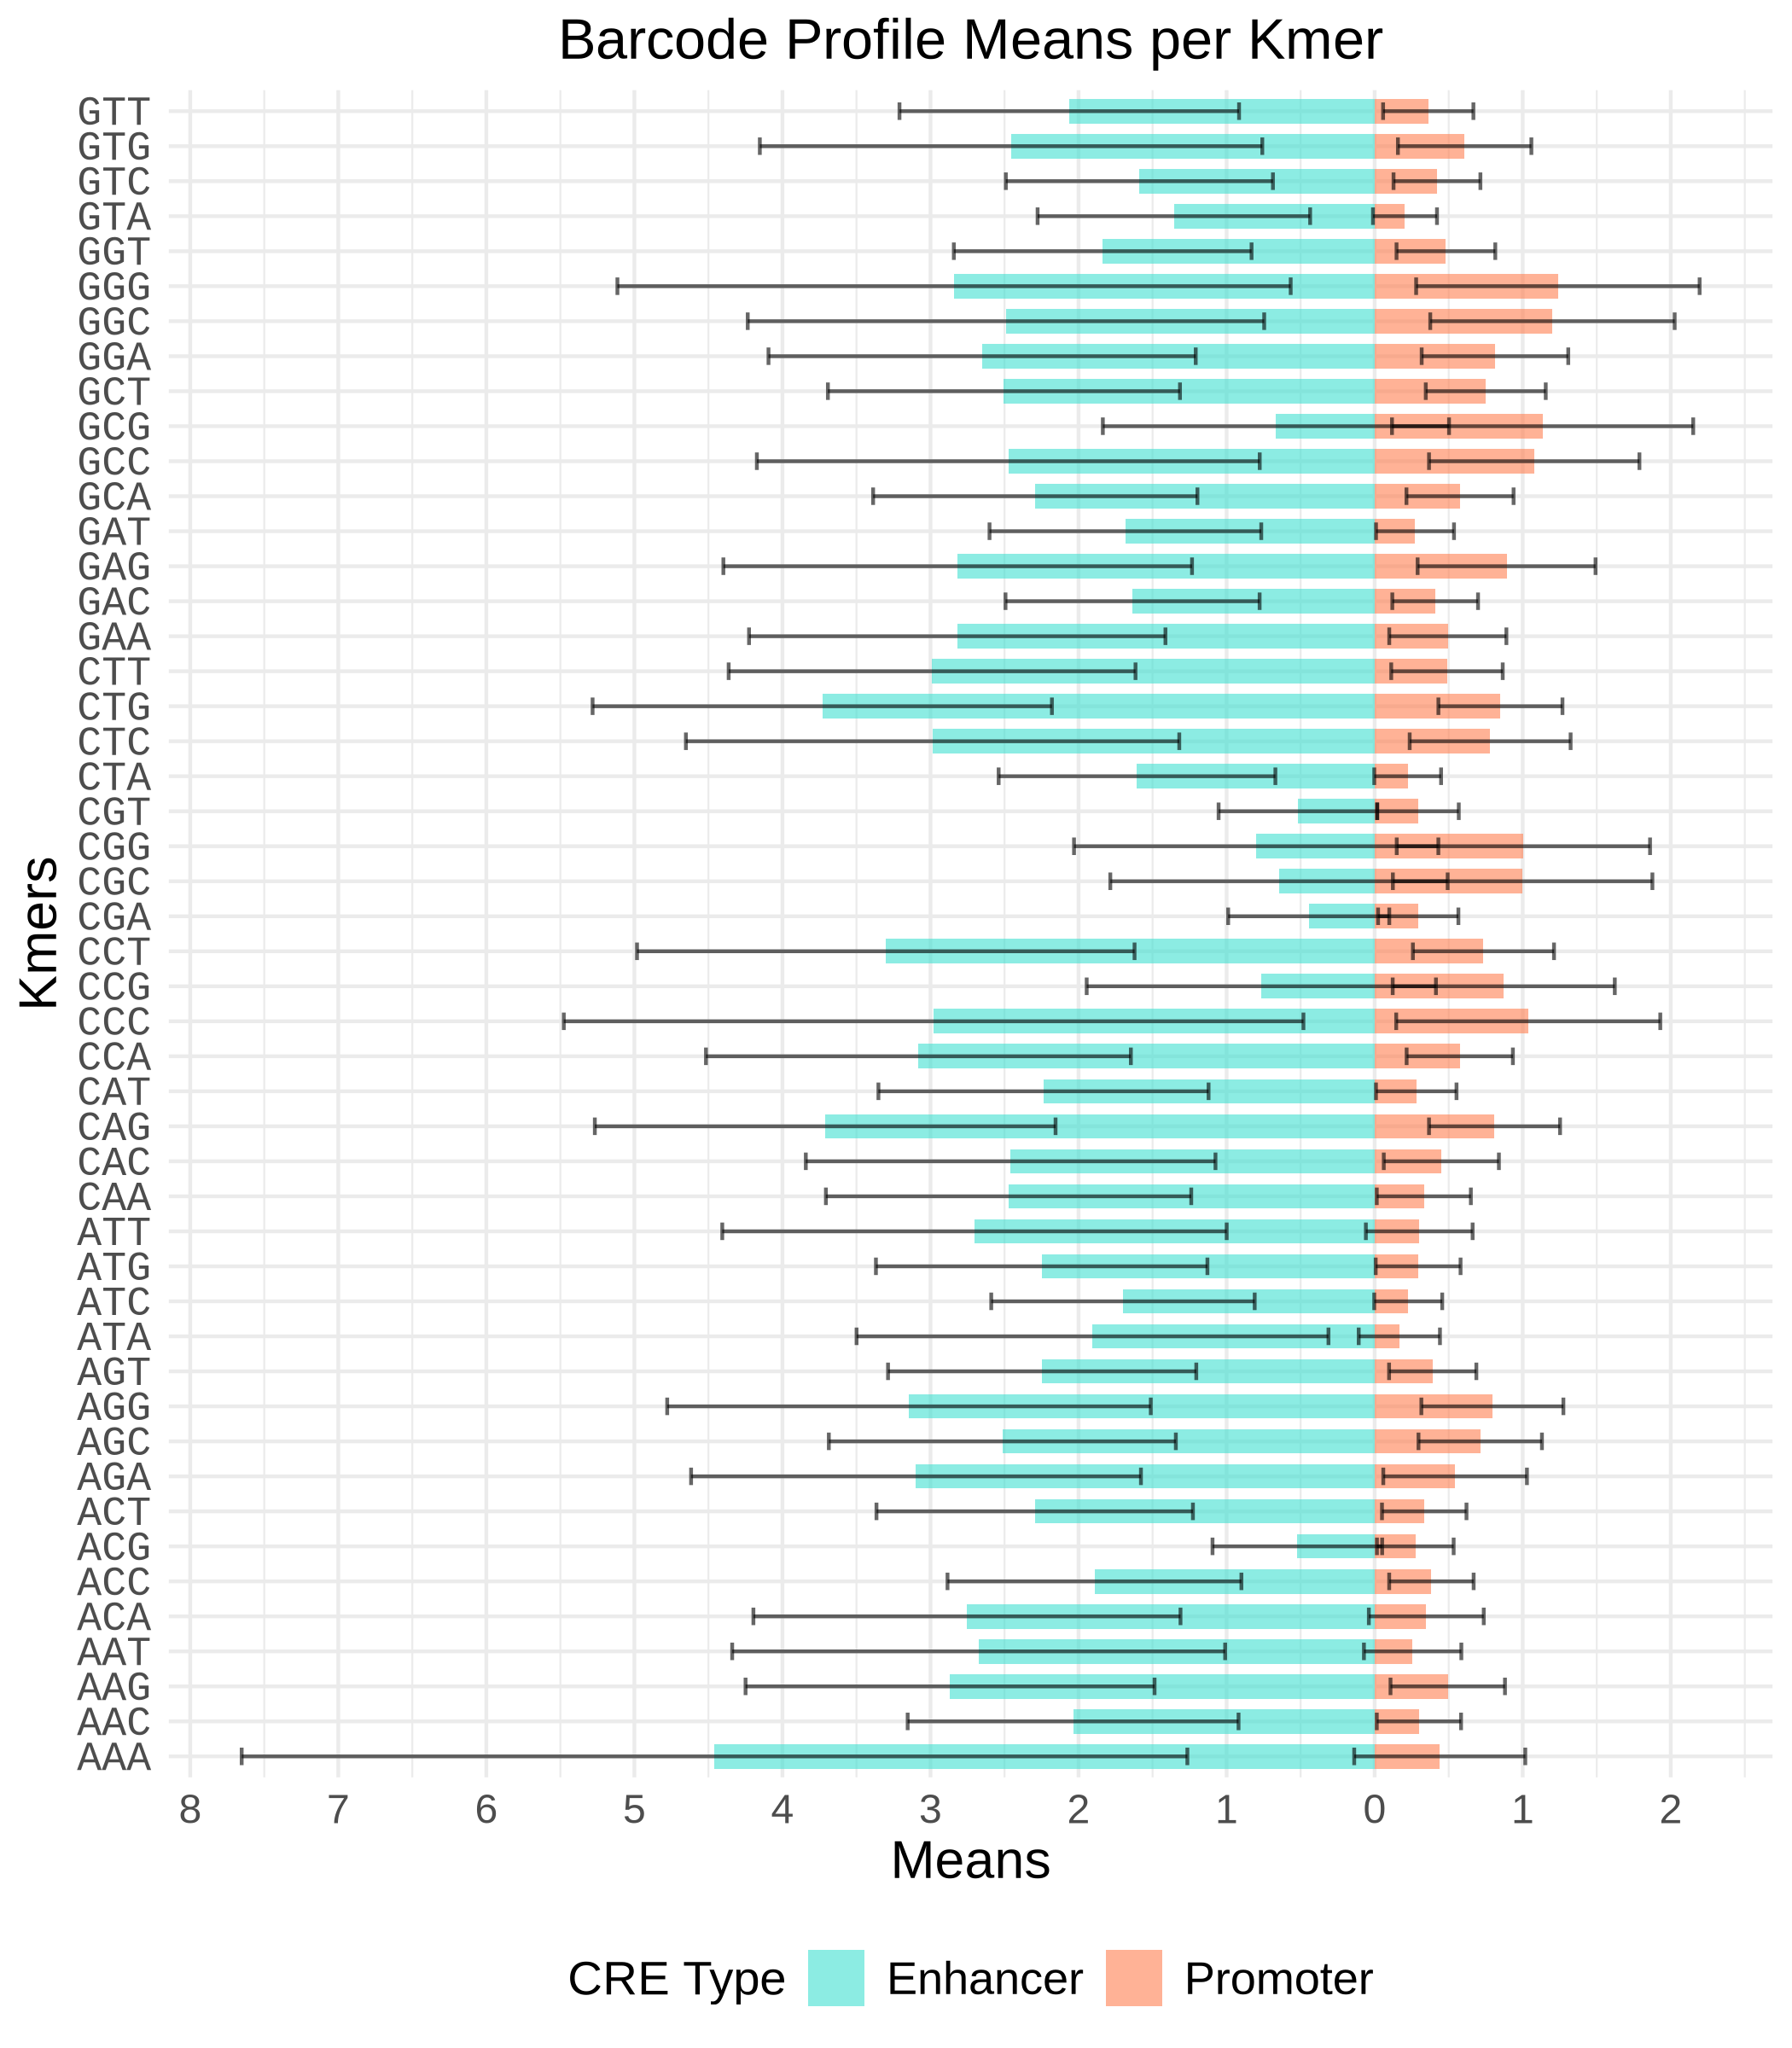
\includegraphics{gb-test-pdf_files/figure-pdf/figure-prods-2.png}
\end{center}




\end{document}
